\documentclass[runningheads]{llncs}
\usepackage[T1]{fontenc}
\usepackage{graphicx}
\usepackage{amsmath}
\usepackage{amssymb}
\usepackage{enumitem}
\usepackage{multirow}
\usepackage{tabularx}
\usepackage{hyperref}
\usepackage{ragged2e}
\usepackage{booktabs} 
\usepackage{subcaption}
\usepackage[misc]{ifsym}
\newcommand{\corr}{(\Letter)}
% N.B.: do not change anything above this line. If you require additional packages, please load them directly after this line.
\usepackage{mwe}
% N.B.: you may delete the preceding line. It is used to display an example image in this template.

\begin{document}

\title{Understanding Implications of Dataset Choice for Feature Effect Estimation:
    A Simulation-Based Investigation through Error Decomposition}

\titlerunning{Understanding Implications of Dataset Choice for Feature Effect Estimation}
% If the full title of your paper is short enough to also fit in the running head, you can omit the abbreviated paper title here. You can check as follows: if you comment out the \titlerunning line, something will appear in the header of all odd-numbered pages of your PDF from page 3 onward. This something is either the full title (in which case all is well), or the error message "Title Suppressed Due to Excessive Length". If this error message appears, you're going to want to provide an abbreviated title within the \titlerunning command, because if you won't do it, Springer will do it for you.

%N.B.: Author information (both in the \author{} and \authorrunning{} command) should only be present in the Camera-Ready Version of your paper. The version that you initially submit for review, ought to be double-blind. So, when initially submitting your paper, use:
%\author{Author information scrubbed for double-blind reviewing}
\author{Timo Heiß\inst{1}}
% You may leave out the orcidID information, if you want to.
% Use \corr to indicate the corresponding author. Note the spacing around the \corr command. Only one author can be the corresponding author.

%N.B.: comment out the \authorrunning{} command for the double-blind version of your paper submitted for review. Later, if your paper is accepted, use the command for the Camera-Ready Version.
\authorrunning{Timo Heiß}
% First names are abbreviated in the running head.
% If there is one author, write 'A.L. Benjamin'.
% If there are two authors, write 'A.L. Benjamin and C.C. Broadus Jr.'
% If there are more than two authors, '[...] et al.' is used.

\institute{Department of Statistics, LMU Munich, Ludwigstr. 33, 80539 Munich, Germany \email{t.heiss@campus.lmu.de}}

\maketitle              % typeset the header of the contribution

\begin{abstract}
    As Machine Learning models are increasingly employed in critical domains
    like healthcare and finance, ensuring accurate model explanations by
    Interpretable Machine Learning methods becomes crucial to avoid misguided
    decisions. The choice of dataset for estimating feature effects --- whether
    to use training data, validation data, or even employ cross-validation ---
    is one important fundamental question in this context that remains largely
    unexplored.
    Through a comprehensive simulation study, we investigate this question for
    Partial Dependence Plots (PDP) and Accumulated Local Effects (ALE), decomposing
    their error into bias and variance components. We extend previous work by
    providing a theoretical framework for error decomposition and contribute
    a systematic overview of test functions for simulation studies in Interpretable ML.  % chktex 13
    Our simulation study results validate the common practice of using training
    data, showing no evidence against it. We find that larger datasets for estimation
    are generally preferable due to reduced Monte Carlo variance, with ALE being
    particularly sensitive to dataset size. Cross-validation emerges as a promising
    approach, reducing both model and Monte Carlo variance, which is especially
    beneficial for overfitting models.
    Our findings enable practitioners to make informed decisions about dataset
    choice for feature effect estimation while establishing a foundation for
    future research in this area.\footnote{Our entire implementation and results
    are available at \url{https://github.com/timo282/current-research-feature-effects}.}

    \keywords{Interpretable Machine Learning  \and Feature effects \and Partial dependence plot \and Accumulated local effects}
\end{abstract}

\section{Introduction}
Most Machine Learning (ML) models can be considered black boxes --- opaque
systems that intrinsically do not allow insight into their internal reasoning,
making it often impossible to explain their decisions. This can be
problematic in many critical domains and applications, such as healthcare,
legal, or finance, where decisions must be transparent and
accountable~\cite{adadi_peeking_2018}.

The need for interpretability in ML stems from multiple factors: building trust in
model predictions~\cite{ribeiro_why_2016,teach_analysis_1981},  identifying and mitigating
potential biases~\cite{guidotti_survey_2019}, addressing fairness and ethical concerns
~\cite{lipton_mythos_2018}, and ensuring compliance with regulations like the
EU's General Data Protection Regulation (GDPR)~\cite{gdpr2016} and AI
Act~\cite{euaia2024}. To address these challenges, the field of Explainable AI
/ Interpretable ML has emerged~\cite{adadi_peeking_2018}, developing a
wide variety of methods to explain ML models. This includes both model-specific and
model-agnostic approaches ranging from local feature attributions to global
feature importances and effects\footnote{For comprehensive overviews of Explainable AI
    methods, see
    e.g.~\cite{adadi_peeking_2018,kamath_introduction_2021,molnar_interpretable_2022}.}.

Due to the severity of many applications, it is crucial to utilize these
interpretability methods correctly to avoid misleading or incorrect conclusions.
In general, there are many pitfalls to be aware of~\cite{molnar_general_2022},
including the question whether to compute explanations in-sample, i.e.\ on training data, or
out-of-sample, which we refer to as validation data in the following. Existing
works have studied the implications of this choice for many methods, including
studies on \textit{Permutation Feature Importance (PFI) }~\cite{molnar_general_2022},
\textit{Mean Decrease in Impurity (MDI)} of
Random Forests~\cite{loecher_debiasing_2022}, or \textit{SHAP}
values~\cite{loecher_debiasing_2024}.

However, to the best of our knowledge, there exist no such systematic studies
for feature effect methods like \textit{Partial Dependence Plots
    (PDP)}~\cite{friedman_greedy_2001} and \textit{Accumulated Local Effects
    (ALE)}~\cite{apley_visualizing_2020}. Current literature
(e.g.,~\cite{apley_visualizing_2020,friedman_greedy_2001,molnar_interpretable_2022})
predominantly uses training data without explicit justification, while
practitioners also advocate for using unseen validation data (for details, see
\textsc{Section~\ref{sec:related-works}}). Factors that may influence this
choice include potential biases arising from overfitting, the dataset size, and
computational constraints. Although PDP and ALE are not based on generalization
error like PFI, it is not studied if and how they are affected by overfitting
when estimated on training data. In addition, larger datasets may improve the
feature effect estimates but also increase computation times.\\

\noindent In this paper, we aim to answer this largely unaddressed, fundamental
methodological question of whether to use training or validation data to
compute feature effects. We perform an empirical simulation study, estimating
PDP and ALE on training data, validation data, and in a cross-validated manner
for different models and dataset. We decompose the error of PDP and ALE and
compare the error components to understand the implications of the data choice.
Our main contributions can be summarized as follows:

\begin{enumerate}
    \item We shed light on the question of whether to compute feature effects on training
          data, validation data, or in a cross-validated manner, grounded through our
          comprehensive simulation study, considering feature effect error, bias, and
          variance across different models and datasets.
    \item We extend previous work to provide a theoretical framework for decomposing
          feature effect errors and estimating the corresponding components.
    \item We provide an overview of commonly used test functions for simulation studies,
          including applications and purposes, as guidance for researchers in
          Interpretable ML. % chktex 13
\end{enumerate}

\noindent These contributions have several important implications: First, our empirically
grounded recommendations enable practitioners and researchers to make informed
decisions about which data to choose for feature effect estimation, helping to
understand potential implications of their choices. Additionally, our framework
for evaluating feature effects and our systematic collection of test functions
provide a foundation for future research in Interpretable ML, with the latter
specifically facilitating test function choice for simulation studies.\\

\noindent The remainder of this paper is structured as follows. In
\textsc{Section~\ref{sec:related-works}}, we provide an overview of related
works on feature effects and test functions for simulation studies. In
\textsc{Section~\ref{sec:background}}, introduce the considered feature
effect methods PDP and ALE, and demonstrate how to decompose the error of these
feature effects, providing corresponding definitions and estimators.
We then describe the methodology and set-up of our simulation studies in
\textsc{Section~\ref{sec:methodology-set-up}}, present the results in
\textsc{Section~\ref{sec:results}}, and conclude our work with a discussion
of their implications and limitations in \textsc{Section~\ref{sec:conclusion}}.

\section{Related Works}\label{sec:related-works}

\subsection{Feature Effects}

\paragraph{Feature Effect Methods.}
Current literature offers various methods for analyzing feature effects in ML.  % chktex 13
One of the most popular methods is the \textit{Partial Dependence Plot
    (PDP)}~\cite{friedman_greedy_2001}, which describes the marginal effect of one
or two features on the model prediction. The PDP assumes that the features of
interest are independent of the remaining features. When this assumption is
violated, the method may produce unrealistic data points outside the underlying
joint data distribution of the data, which can cause misleading
interpretations (``extrapolation issue'')~\cite{molnar_interpretable_2022,molnar_general_2022}.

\textit{M-Plots (Marginal Plots)} try to address this issue by considering the
conditional distribution of the remaining features given the feature of interest
but instead suffer from the omitted variable
bias~\cite{apley_visualizing_2020,friedman_greedy_2001}.

The \textit{Accumulated Local Effects (ALE)} plot~\cite{apley_visualizing_2020}
addresses both issues by accumulating local differences in model predictions
along the feature of interest, computing conditional expectations within small
intervals rather than across the entire feature range.

Alternative approaches include \textit{functional ANOVA (fANOVA)}, which
decomposes feature effects into main and interaction
effects~\cite{hooker_discovering_2004}. Recent extensions have further
addressed limitations of the methods above: \textit{Robust
    and Heterogeneity-aware ALE (RHALE)}~\cite{gkolemis_rhale_2023} adds
heterogeneity quantification to ALE and improves robustness.
\textit{Accumulated Total Derivative Effect (ATDEV)} plots can be decomposed
into ALE and \textit{Accumulated Cross Effects (ACE)}~\cite{liu_model_2018}.

Beyond these global feature effect methods, there are regional effect plots
such as \textit{REPID}~\cite{herbinger_repid_2022}, and local methods like
\textit{ICE (Individual Conditional Expectation)}
curves~\cite{goldstein_peeking_2015} or SHAP dependence
plots~\cite{lundberg_local_2020}.

In the following, we focus on PDP and ALE and refer to them when speaking of
feature effects.

\paragraph{Feature Effect Error and Uncertainty.}
Multiple works have approached measuring uncertainty in feature effects. For
probabilistic ML models, Moosbauer et al.\cite{moosbauer_explaining_2021}
derived model-specific confidence bands for PDPs, while applied studies have
proposed bootstrap-based
approaches~\cite{esselman_landscape_2015,grange_using_2019}. While the former
are not model-agnostic, the latter often capture only the variance introduced
by Monte Carlo approximation. However, the model variance is another source
of uncertainty in PDPs and ALEs, and accounting for it requires multiple model
fits~\cite{apley_visualizing_2020,molnar_general_2022}.

Molnar et al.~\cite{molnar_relating_2023} give formalizations of PDP (and PFI)
as statistical estimators of ground truth estimands, demonstrate the
decomposition of its mean squared error (MSE) into model bias, model variance,
and Monte Carlo variance, and provide estimators for both Monte Carlo and
overall variance. Our work builds upon and extends this idea.

\paragraph{Data Choice for Feature Effect Estimation.}
For many interpretability methods, the choice whether to compute explanations
in-sample (on training data) or out-of-sample (on validation data) can
significantly impact interpretations: For loss-based methods such as
\textit{Permutation Feature Importance (PFI)
}\cite{breiman_random_2001,fisher_all_2019}, this choice is crucial and has
been extensively studied (e.g., in~\cite{molnar_general_2022}). Similar
concerns have been identified for other explainability methods: both the
\textit{Mean Decrease in Impurity (MDI)} of Random Forests and \textit{SHAP}
values have been shown to potentially exhibit biases when computed on training
data~\cite{loecher_debiasing_2022,loecher_debiasing_2024}.

For feature effect methods, however, the implications of this choice remain
largely unexplored. The original works introducing
PDP~\cite{friedman_greedy_2001} and ALE~\cite{apley_visualizing_2020}, as well
as general introductory literature on Interpretable
ML~\cite{molnar_interpretable_2022}, predominantly use training data without
explicit justification. In contrast, practitioners often advocate for using
holdout data or base their choice on practical constraints such as dataset
size\footnote{for examples, see
    \url{https://github.com/SauceCat/PDPbox/issues/68} and
    \url{https://forums.fast.ai/t/partial-dependence-plot/98465} (both accessed
    10/27/2024)}. A too large dataset can increase computation times substantially,
particularly for PDPs~\cite{friedman_greedy_2001}. Moreover, Molnar et
al.~\cite{molnar_relating_2023} estimate the PDP on holdout data when aiming to
quantify the variance of feature effect estimates. Nonetheless, a systematic
study on the implications of the data choice for feature effect estimation is
missing so far.

\subsection{Test Functions for Simulation Studies}\label{sec:test-functions}

Test functions play a crucial role in research, e.g.\ for evaluating different
methodological approaches, or when conducting simulation studies. In the
following, we synthesize commonly used test functions across various domains,
providing structured guidance for researchers, particularly those in
Interpretable ML, in selecting appropriate test functions to facilitate
designing simulation studies.

\paragraph{Test Functions in Optimization.}
The field of optimization, where test functions are essential to enable the
assessment and comparison of optimization algorithms, has established a rich
foundation of test functions. A fundamental approach involves using simple
mathematical expressions like the sphere function~\cite{more_testing_1981}.
These basic functions are often combined with more complex ones like Branin or
Rosenbrock to create comprehensive test suites that incorporate important
properties such as nonlinearity, non-separability, and
scalability~\cite{whitley_building_1998}. A notable framework in this domain is
the Comparing Continuous Optimizer (COCO) platform with its Black Box
Optimization Benchmark (BBOB), offering a structured approach to testing
continuous optimization algorithms through artificial test
functions~\cite{hansen_coco_2016}. While being
well-established in optimization, they may also serve as a basis for
Interpretable ML researchers. However, the ability of these artificial test
functions to represent complex real-world behavior is
limited~\cite{zaefferer_simulation-based_2017}.

\paragraph{Physics-Inspired Test Functions.}

Physics-derived functions offer a compelling source of real-world test cases,
with the \textit{Feynman Symbolic Regression Database
    (FSReD)}~\cite{udrescu_ai_2020} as a prominent example. FSReD comprises 100
physics equations from the seminal \textit{Feynman's Lectures on Physics
    (34--36)}, supplemented by 20 more challenging equations from other seminal
physics texts. These equations span diverse physics domains and involve a
varying number of variables and various elementary functions. Tabular datasets are
generated through random sampling from defined value ranges.

Matsubara~et~al.~\cite{matsubara_rethinking_2024} addressed several limitations
of the original FSReD by introducing a three-tiered categorization of problems
based on their complexity, incorporating dummy variables to
simulate irrelevant features, and implementing more realistic sampling ranges and
strategies. Detailed specifications for all formulas, including their sampling
parameters, are available in their work.

While originally designed for symbolic regression tasks, many Feynman equations
serve as suitable test functions for simulation studies in Interpretable
ML. Their basis in physical principles provides real-world relevance, though  % chktex 13
researchers should carefully select equations that align with their specific
analytical objectives and complexity requirements.

\paragraph{Test Functions for Interpretable Machine Learning.}
The Interpretable ML field itself has developed several specialized test
functions designed to evaluate specific aspects of interpretability methods.
Goldstein et al.~\cite{goldstein_peeking_2015} used several simple test
functions to demonstrate the behavior of Individual Conditional Expectation
(ICE) curves. These include a simple additive function to demonstrate the
absence of interactions, simple interactions to reveal heterogeneity that might
be obscured by PDPs, and a specially designed
function with an empty quadrant for assessing extrapolation behavior.

Similarly, Liu et al.~\cite{liu_model_2018} focused on simple functions before
increasing complexity. They started with basic two-variable scenarios
--- additive functions, interaction functions, and combinations thereof
--- and examined these under both independent and correlated features,
comparing various feature effect methods. Advantages of these simple test
functions are that solutions (e.g., feature effects) can be computed
analytically, and that they allow for more fine-grained analyses of
individual aspects.

A more complex test function suite was proposed by
Tsang~et~al.~\cite{tsang_detecting_2017}, specifically designed to evaluate the
detection of variable interactions. Their functions incorporate various types
of interactions with different orders, strengths, non-linearities, and
overlaps. While being particularly valuable for interaction 
detection, they are also useful for evaluating other interpretability methods
in scenarios with complex interactions.

The Friedman functions~\cite{breiman_bagging_1996,friedman_multivariate_1991}
serve as classical benchmarks applicable across various interpretability tasks.
These three functions combine linear and non-linear effects with interactions,
incorporating dummy variables and random noise terms to reflect realistic
complexity. For detailed specifications, see~\cite{breiman_bagging_1996}.

When choosing test functions for simulation studies in Interpretable ML,
researchers should consider several criteria, including the specific aspects of
interpretability being evaluated, the desired complexity level and number of
variables, the presence of specific challenges such as correlation between
features or interactions, the need for analytical solutions for validation, as
well as the relevance to real-world applications.

\section{Theoretical Framework: Feature Effects and Error Decomposition}\label{sec:background}

\subsection{Feature Effects}

The \textit{Partial Dependence Plot (PDP)}~\cite{friedman_greedy_2001} describes the marginal effect of one or
two features on the prediction of a model $\hat f$. For a feature set $X_S$
(with $S \subseteq \{1,\ldots,p\}$, $|S| = 1$ or $|S| = 2$), the PDP is defined
as

\begin{equation}
    PDP_{\hat f, S} = \mathbb{E}_{X_C}[\hat{f}(x_S, X_C)] = \int \hat f(x_S, x_C)d\mathbb{P}(x_C),
\end{equation}

\noindent where $X_C$ is the complement feature subset. $PDP_{\hat f, S}$ is a
function of $x_S$ and can be estimated by Monte Carlo integration:

\begin{equation}\label{eq:pdp-estimate}
    \widehat{PDP}_{\hat f, S}(x_S) = \frac{1}{n} \sum_{i=1}^{n} \hat{f}(x_S, x_C^{(i)}).
\end{equation}

\noindent Here, $x_C^{(i)}$ are the actual complement feature values from the dataset of $n$ instances.
To plot the function, a grid of $G$ grid points
$\{(x_S^{(g)}, \widehat{PDP}_{\hat f, S}(x_S^{(g)}))\}_{g=1}^G$ can be used~\cite{molnar_relating_2023}.  % chktex 3
Molnar et al.~\cite{molnar_general_2022} recommend using quantile-based over equidistant grids.\\

\newpage
\noindent The \textit{Accumulated Local Effects (ALE)} plot~\cite{apley_visualizing_2020}
for $|S|=1$ is defined as

\begin{eqnarray}
    ALE_{\hat f,S}(x_S) &=& \int_{x_{\text{min},s}}^{x_S} \mathbb{E}_{X_C|X_S}
    \left[\hat{f}^S(X_S, X_C)|X_S = z_S\right] dz_S - \text{constant} \\
    &=& \int_{x_{\text{min},s}}^{x_S} \int_{x_C}
    \hat{f}^S(z_S, x_C)\mathbb{P}(x_C|z_S)dx_{C}dz_{S} - \text{constant},
\end{eqnarray}

\noindent where $\hat{f}^S(x_S, x_C) = \frac{\partial \hat{f}(x_S, x_C)}{\partial x_S}$.
The constant is chosen so that $ALE_{\hat f,S}(X_S)$ is centered with a mean of $0$
w.r.t.\ the marginal distribution of $X_S$. The uncentered ALE can be estimated by

\begin{equation}\label{eq:ale-estimate-uncentered}
    \widehat{\widetilde{ALE}}_{\hat f, S}(x) =
    \sum_{k=1}^{k_S(x)} \frac{1}{n_S(k)} \sum_{i:x_S^{(i)} \in N_S(k)}
    \left[\hat f(z_{k,S}, x_{C}^{(i)}) - \hat f(z_{k-1,S}, x_{C}^{(i)})\right].
\end{equation}

\noindent Here, $\{N_S(k) = (z_{k-1,S}, z_{k,S}]\}_{k=1}^{K}$ partitions the samples  % chktex 3 chktex 9
$\{x^{(i)}_S\}_{i=1}^n$ into $K$ intervals or neighborhoods $N_S(k)$. $n_S(k)$ denotes  % chktex 3
the number of observations in the $k$th interval, $k_S(x)$ the index
of the interval to which a particular value $x$ of feature $S$ belongs.
The uncentered ALE is centered by

\begin{equation}\label{eq:ale-estimate-centered}
    \widehat{ALE}_{\hat f, S}(x) =
    \widehat{\widetilde{ALE}}_{\hat f, S}(x)
    - \frac{1}{n} \sum_{i=1}^n \widehat{\widetilde{ALE}}_{\hat f, S}(x_S^{(i)})
\end{equation}

\noindent to have a mean effect of $0$. For the grid that defines the intervals,
the quantiles of the empirical distribution of $\{x^{(i)}_S\}_{i=1}^n$ can be  % chktex 3
used~\cite{apley_visualizing_2020}.

\subsection{Feature Effect Error Decomposition}

\paragraph{Feature effect ground truth.} To quantify the error of a computed
feature effect, a ``ground truth'' needs to
be defined first. We follow the approach of Molnar et
al.~\cite{molnar_relating_2023} and define ground truth versions of PDP and ALE
directly on the data generating process (DGP) by applying PDP and ALE to the
underlying ground truth function $f$ (instead of model $\hat f$).
For PDP, we can directly use the definition of Molnar et
al.~\cite{molnar_relating_2023}:

\begin{definition}[Definition 1 from~\cite{molnar_relating_2023}]
    The PDP ground truth is the PDP applied to function
    $f : \mathcal{X} \xrightarrow{} \mathcal{Y}$
    of the data generating process.

    \begin{equation}
        PDP_{f,S}(x_S) = \mathbb{E}_{X_C}[f(x_S,X_C)]
    \end{equation}
\end{definition}

\noindent As stated by Molnar et al.~\cite{molnar_relating_2023}, their results also
apply to conditional variants of the PDP such as ALE. We now make this  % chktex 13
definition explicit.

\newpage

\begin{definition}
    The ALE ground truth is the ALE applied to function $f : \mathcal{X} \xrightarrow{} \mathcal{Y}$ of the data generating process.

    \begin{equation}
        ALE_{f,S}(x_S) = \int_{x_{\text{min},s}}^{x_S} \mathbb{E}_{X_C|X_S} \left[f^S(X_S, X_C)|X_S = z_S\right] dz_S - \text{constant}
    \end{equation}

    \noindent where $f^S(x_S, x_C) = \frac{\partial f(x_S, x_C)}{\partial x_S}$ and \text{constant} chosen such that the effect has a mean of $0$ w.r.t.\ the marginal distribution of $X_S$.
\end{definition}

%With these definitions, $\widehat{PDP}_{\hat f,S}$ and $\widehat{ALE}_{\hat f,S}$
%can now be treated as statistical estimators of the ground truth feature effects
%(cf.~\cite{molnar_relating_2023}). 
\noindent Note that different ground truth feature effects can also be defined, and our choices
come with certain implications and limitations, such as omitting the
\textit{aggregation bias}~\cite{herbinger_repid_2022,mehrabi_survey_2021}.

With more complex ground truth functions $f$, it becomes often infeasible to
derive the ground truth feature effects analytically. For these cases, we
therefore propose to also estimate those effects by  % chktex 13
Monte Carlo integration, yielding $\widehat{PDP}_{f,S}(x_S)$ and
$\widehat{ALE}_{f,S}(x_S)$ (obtained by plugging $f$ instead of $\hat f$
into the estimators in equations (\ref{eq:pdp-estimate}) and
(\ref{eq:ale-estimate-uncentered}) / (\ref{eq:ale-estimate-centered})).

\paragraph{Feature effect error decomposition.} Summarizing, we have now defined four quantities per feature effect:
$PDP_{f,S}$ $\widehat{PDP}_{f,S}$, $PDP_{\hat f,S}$, and $\widehat{PDP}_{\hat f,S}$
(analogously for ALE). Between these quantities, different error metrics can because
defined. In this paper, we focus on MSE as it can be decomposed into
bias and variance~\cite{geman_neural_1992}.
When taking $PDP_{f,S}$ as ground truth, the MSE of $PDP_{\hat f,S}$ at
point $x_S$ can be formulated as follows~\cite{molnar_relating_2023}:

\begin{equation}
    \text{MSE}(x_S; PDP_{f,S}, PDP_{\hat f,S})
    = \mathbb{E}_F[{(PDP_{f,S}(x_S) - \widehat{PDP}_{\hat f,S}(x_S))}^2]
\end{equation}
\begin{equation}
    = \underbrace{{(PDP_{f,S}(x_S) - \mathbb{E}_F[PDP_{\hat{f},S}(x_S)])}^2}_{Bias^2} + \underbrace{\text{Var}_F[PDP_{\hat{f},S}(x_S)]}_{Variance}
\end{equation}

\noindent Here, $F$ denotes the distribution of trained models. The bias
is linked to the bias of the model, the variance comes from the variance
in the model fits (randomness in training data, randomness in model training procedure).

Since we usually cannot determine $PDP_{\hat f,S}$, we need to estimate it by
Monte Carlo integration, which introduces an additional variance term (we use the random variable
$X$ for the Monte Carlo samples):

\begin{equation}
    \begin{split}
        \text{MSE}(x_S; PDP_{f,S}, \widehat{PDP}_{\hat f,S})
        = \underbrace{{(PDP_{f,S}(x_S) - \mathbb{E}_F[PDP_{\hat{f}, S}(x_S)])}^2}_{Bias^2} \\
        + \underbrace{\text{Var}_F[PDP_{\hat{f},S}(x_S)]}_{Variance} + \underbrace{\mathbb{E}_F\text{Var}_{X}[\widehat{PDP}_{\hat{f},S}(x_S)]}_{MC-Variance}
    \end{split}
    \label{eq:mse-decomposition}
\end{equation}

\begin{proof}
    Using basic expectation and variance rules, as well as applying the fact that
    $\mathbb{E}_X[\widehat{PDP}_{\hat f}] = PDP_{\hat f}$ (cf.~\cite{molnar_relating_2023})
    gives the proof. The full proof is provided in
    \textsc{Appendix~\ref{app:proof-mse-decomposition}}.
\end{proof}

\noindent We see that the variance due to MC integration also depends on the model
distribution $F$. Similarly, one could use the estimate $\widehat{PDP}_{f,S}$
as ground truth, introducing an additional variance term when
estimated with Monte Carlo samples (proof in
\textsc{Appendix~\ref{app:proof-mc-variance}}).
An overview of all error terms is given in
\textbf{Fig.\@~\ref{fig:error-graph}}.

\begin{figure}[t]
    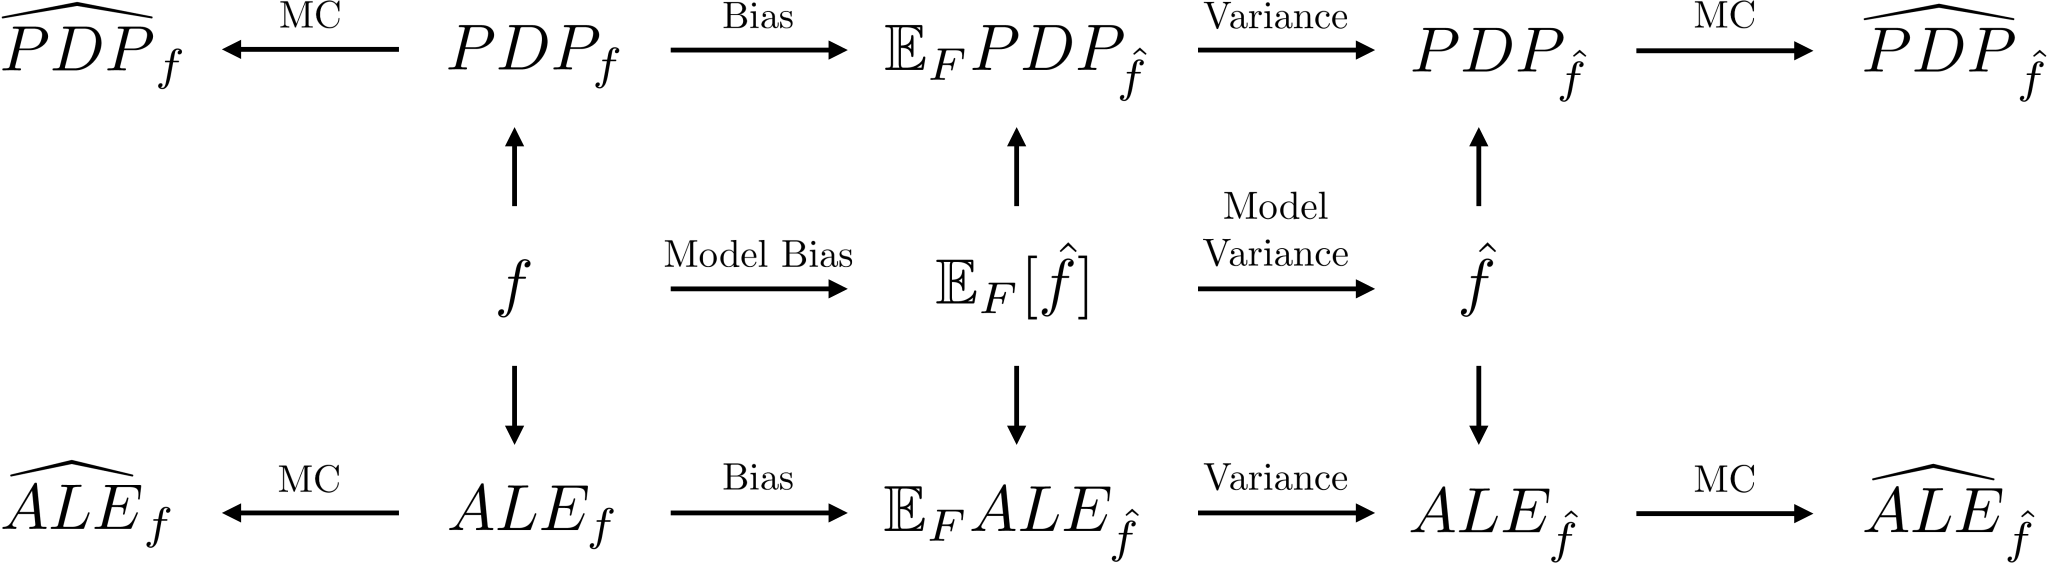
\includegraphics[width=\textwidth]{img/error_graph.pdf}
    \caption{Error chain in feature effect estimation. The deviation of the estimated
        feature effect from the ground truth can be decomposed into bias, model variance,
        and Monte Carlo variance. If the ground truth is estimated by Monte Carlo
        integration, an additional Monte Carlo variance term arises. This graphic
        builds on~\cite{molnar_relating_2023}.}\label{fig:error-graph}
\end{figure}

\paragraph{Feature effect error estimation.} Next, we aim to estimate these error terms.
$\mathbb{E}_F$ and $\text{Var}_F$ can be estimated by averaging over
multiple models of the same inducer fitted to $M$ different training data
sets, each independently sampled from the DGP. We propose the following estimators:  % chktex 13

\begin{equation}
    \widehat{\text{MSE}}(x_S; PDP_{f,S}, \widehat{PDP}_{\hat f,S}) = \frac{1}{M} \sum_{m=1}^{M} {(PDP_{f,S}(x_S) - \widehat{PDP}_{\hat f^{(m)},S}(x_S))}^2
    \label{eq:mse-estimator}
\end{equation}
\begin{equation}
    \widehat{\text{Bias}}(x_S; PDP_{f,S}, \widehat{PDP}_{\hat f,S}) = (PDP_{f,S}(x_S) - \frac{1}{M}\sum_{m=1}^M \widehat{PDP}_{\hat{f}^{(m)},S}(x_S))
    \label{eq:bias-estimator}
\end{equation}
\begin{equation}
    \begin{split}
    \widehat{\text{Variance}}(x_S; \widehat{PDP}_{\hat f,S}) = \\
    \frac{1}{M-1}\sum_{m=1}^M{\left(\widehat{PDP}_{\hat f^{(m)},S}(x_S) - \frac{1}{M}\sum_{m=1}^M \widehat{PDP}_{\hat f^{(m)},S}(x_S)\right)}^2
    \end{split}
    \label{eq:variance-estimator}
\end{equation}

\noindent The variance estimator is the same as in~\cite{molnar_relating_2023},
capturing both the variance in the model fits and the variance due to
MC integration. For the Monte Carlo variance of estimating the ground truth by
Monte Carlo integration, i.e.\ omitting the model, we propose the following estimator:
\begin{equation}
    \widehat{\text{Variance}}_{MC}(x_S; PDP_f, \widehat{PDP}_f) = \frac{1}{K}\sum_{k=1}^K{(PDP_f(x_S) - \widehat{PDP}_f^{(k)}(x_S))}^2
    \label{eq:mc-variance-estimator-groundtruth}
\end{equation}

\noindent To estimate the Monte Carlo variance for feature effects of models
given in equation~\ref{eq:mse-decomposition}, we have to consider multiple
Monte Carlo iterations for multiple model refits, yielding the following estimator:

\begin{equation}
    \begin{split}
        \widehat{\text{Variance}}_{MC}(x_S; \widehat{PDP}_{\hat{f}}) = \\ \frac{1}{M(K-1)}\sum_{m=1}^M \sum_{k=1}^K
        {\left(\widehat{PDP}_{\hat f^{(m)},S}^{(k)}(x_S) - \frac{1}{K}\sum_{k=1}^K \widehat{PDP}_{\hat f^{(m)},S}^{(k)}(x_S)\right)}^2
    \end{split}
    \label{eq:mc-variance-estimator-model}
\end{equation}

\noindent While these estimators are based on the PDP, they
can be defined analogously for ALE.  % chktex 13
% For a more convenient analysis of the errors, we suggest
% an aggregation of the error terms over the marginal distribution of $X_S$
% (e.g., by averaging over the grid points if chosen appropriately)
% to obtain a single error measure per feature effect.
It is important to note that most of these estimators are rather
impractical as they require knowledge of the ground truth. Nonetheless,
we rather use them to understand the behavior of the feature
effect error components under different dataset choices. This
distinguishes our approach from previous works such as~\cite{molnar_relating_2023},
which mostly focus on providing practical variance estimates to provide
confidence intervals for uncertainty quantification in feature effects. 


\section{Methodology \& Experimental Set-Up}\label{sec:methodology-set-up}

To address the central research question of this paper, which data to
choose for feature effect estimation, we conduct a comprehensive simulation
study. For different models,
datasets, and dataset sizes, we estimate the feature effects PDP and ALE on
training data, validation data, and in a cross-validated manner. We then
compute the feature effect error as MSE against the ground truth
feature effects, and decompose it into bias and variance components. By
comparing these error terms across the different estimation strategies
(training, validation, cross-validation), we aim to provide nuanced empirical
insights into the implications of the data choice on feature effect estimation.
To deepen our analysis, we conduct two ablation studies: (1)~decomposing feature
effect variance into model variance and Monte Carlo variance, and (2)~examining
the influence of dataset size on Monte Carlo variance.
In the following, we describe our experimental set-up for the main simulation
study (\textsc{Section~\ref{sec:experiment-main}}) and the ablation studies
(\textsc{Section~\ref{sec:experiment-ablation}}).

\subsection{Main Experiment}\label{sec:experiment-main}

\paragraph{Datasets.}
Building upon \textsc{Section~\ref{sec:test-functions}}, we employ three
distinct datasets of varying complexity for our simulation study:

\begin{itemize}[label=--]
    \item \textbf{SimpleNormalCorrelated} consists of four
          standard-normally distributed features, where the first two
          are strongly correlated ($\rho = 0.9$) while the others are
          independent dummy variables. The target variable is given by:
          \begin{equation}
              f_1(\boldsymbol{x}) = x_1 + \frac{x_2^2}{2} + x_1 x_2
          \end{equation}
          This test function, inspired by~\cite{liu_model_2018}, focuses
          on investigating the impact of correlation and interactions.
    \item \textbf{Friedman1} implements the classical Friedman1 benchmark
          function~\cite{breiman_bagging_1996,friedman_multivariate_1991}
          with seven mutually independent, uniformly distributed features
          between 0 and 1:
          \begin{equation}
              f_2(\boldsymbol{x}) = 10 \sin(\pi x_1 x_2) + 20{(x_3 - \frac{1}{2})}^2 + 10 x_4 + 5 x_5
          \end{equation}
          This dataset includes a mix of linear and non-linear effects with
          interactions.
    \item \textbf{Feynman I.29.16} is based on the Feynman equation I.29.16
          describing wave interference, comprising six independent features. Following
          the refined sampling strategies from Matsubara et al.~\cite{matsubara_rethinking_2024},
          we use two log-uniformly distributed variables on $[0.1, 10]$, two angles uniformly
          distributed over $[0, 2\pi]$, and two uniformly distributed dummy variables on [0,1]:
          \begin{equation}
              f_3(\boldsymbol{x}) = \sqrt{x_1^2 + x_2^2 + 2 x_1 x_2 \cos(\theta_1 - \theta_2)}
          \end{equation}
          This dataset is designed to reflect a physics-based relationship for enhanced real-world relevance.

\end{itemize}

\noindent To generate the datasets, we add a standard-normally distributed noise term $\epsilon$ to each function,
scaled by a signal-to-noise ratio of five\footnote{To determine the noise scaling factor,
    we compute the standard deviation of the signal over 100,000 randomly drawn samples of $y$ and
    divide by the signal-to-noise ratio of five.}. For each test function, we consider two dataset sizes:
$(n_{train}=1000, n_{val}=250)$ and $(n_{train}=8000, n_{val}=2000)$.

\paragraph{Models.}
We consider a set of seven complementary learners, spanning different modeling
paradigms:

\begin{itemize}[label=--]
    \item \textbf{LinReg}: a simple linear regression model as a baseline.
    \item \textbf{GAM\_OT}: a Generalized Additive Model (GAM) with spline terms
          and tensor splines for first-order interactions, number of splines
          and penalization optimally tuned.
    \item \textbf{GAM\_OF}: as above, but with hyperparameters chosen to overfit.
    \item \textbf{SVM\_OT}: a Support Vector Machine (SVM) with optimally tuned hyperparameters.
    \item \textbf{SVM\_OF}: a Support Vector Machine (SVM) with hyperparameters chosen to overfit.
    \item \textbf{XGBoost\_OT}: an XGBoost model with optimally tuned hyperparameters.
    \item \textbf{XGBoost\_OF}: an XGBoost model with hyperparameters chosen to overfit.
\end{itemize}

\noindent Hyperparameters are pre-selected, i.e.\ carefully hand-picked for overfitting scenarios
and tuned on a different dataset for optimal tuning. Details on the hyperparameters and performances
of the models can be found in \textsc{Appendix~\ref{app:model-hps-perf}}.

\paragraph{Feature effect estimation.}
For the trained models, we estimate the feature effects
$\widehat{PDP}_{\hat{f},S}$ and $\widehat{ALE}_{\hat f,S}$ per feature using
equations~(\ref{eq:pdp-estimate}) and (\ref{eq:ale-estimate-uncentered}). For
Monte Carlo integration, we use for each the full training and validation set
as well as a cross-validation strategy. In the latter case, we use a 5-fold
cross-validation on the combined samples of training and validation set, in
each fold fit the model on four folds, and estimate the feature effects on the
remaining fold. We then average the feature effects point-wise over all folds.

We also estimate the ground truth feature effects $\widehat{PDP}_{f,S}$ and
$\widehat{ALE}_{f,S}$ as the complexity of the Feynman equation makes
an analytical computation infeasible. For their Monte Carlo integration, we use
10,000 samples additionally drawn from the DGP, which introduces only a
negligible additional variance as we show in (Section~\ref{sec:results-dataset-size}). We use 100 grid
points, defined by the quantiles of the theoretical distribution of $X_S$ to
enable a comparison across feature effects. Additionally, we center the curves
after estimation to have a mean effect of $0$ w.r.t.\ the grid points, and we
omit the first and the last grid point after estimation to avoid boundary
effects particularly occuring in ALE plots.

\paragraph{Feature effect errors.} To quantify the error of the estimated feature effects, we compute the MSE of
the estimated model feature effects against the estimated ground truth effects,
as well as their bias and variance. We use the
estimators defined in equations~(\ref{eq:mse-estimator}) to
(\ref{eq:variance-estimator}), using $\widehat{PDP}_{f,S}$ instead of
$PDP_{f,S}$ as ground truth (analogously for ALE). We repeat each
dataset-size-model combination $M=30$ times to estimate the error terms, where
each repetition involves drawing a new training and validation set from the
DGP, refitting the models, and estimating the feature effects. To aggregate the
errors into a single number per feature effect, we average them over the
marginal distribution of $X_S$ by averaging over the grid points.

\subsection{Ablation Experiments}\label{sec:experiment-ablation}

As described earlier, we conduct two ablation studies for more detailed
insights into the Monte Carlo variance.

\paragraph{Variance decomposition study.} The variance of the feature effects
estimated in the main experiment \textsc{Section~\ref{sec:experiment-main}} consists of two
components: model variance and variance due to the Monte Carlo
integration. To disentangle these two sources of variance, we estimate the
Monte Carlo variance using the estimator in
equation~(\ref{eq:mc-variance-estimator-model}). By subtracting this from the
total variance obtained in the main experiment, we derive the model variance,
providing more nuanced insights into the implications of data choice in feature
effect estimation. 

For this analysis, we maintain the set-up of the main experiment with one key
modification: for each trained model $\hat f^{(m)}$ (plus the five
models $\hat f^{(m,1)} - \hat f^{(m,5)}$ trained in cross-validation), we draw $K=30$ new training
and validation sets from the DGP. We then estimate feature effects on these  % chktex 13
sets and in a cross-validated manner using the already fitted models. This approach
allows us to estimate the Monte Carlo variance.

Due to the computational intensity of this analysis, we focus only on XGBoost models
(both OT and OF variants), which represent the arguably most practically relevant models
in our setup.

\paragraph{Impact of dataset size on Monte Carlo variance.}
To investigate how dataset size influences Monte Carlo variance,
we estimate the variance between analytical ground truth feature effects
and estimated ground truth feature effects across different dataset sizes.
We use equation~(\ref{eq:mc-variance-estimator-groundtruth}) as estimator
for the Monte Carlo variance. This approach entirely omits the model, thereby
eliminating other error sources such as model bias and variance (simulating a perfect model fit)

We analyze 50 different dataset sizes ranging from $10^1$ to $10^6$ on a logarithmic
scale. We restrict this analysis to the SimpleNormalCorrelated and Friedman1 datasets,
as analytical computation of FeynmanI.29.16 ground truth feature effects is infeasible.
All other experimental details follow the setup of the main experiment.

\section{Results}\label{sec:results}

\subsection{Main Experiment}

We give the results of the main experiment error decomposition for the
SimpleNormalCorrelated dataset in \textbf{Fig.\@~\ref{fig:pdp-results-snc}} for
PDP and \textbf{Fig.\@~\ref{fig:ale-results-snc}} for ALE. The full results for  % chktex 13
all datasets, models, and features can be found in
\textsc{Appendix~\ref{app:additional-results}}.

Generally, we observe that the feature effect error is in the most cases
highest when the effect is estimated on validation data. For ALE, this
observation is more pronounced than for PDP. This increase in error is mainly  % chktex 13
due to an increase in variance (see e.g.,
\textbf{Fig.\@~\ref{fig:pdp-results-snc-gam-ot}} or
\textbf{Fig.\@~\ref{fig:ale-results-snc-xgboost-of}}). For many models, the
feature effect error is lowest when estimated in a cross-validated manner. This
is slightly more pronounced for overfitting models (OF) than for optimally
tuned models (OT), and is mainly due to a decrease in variance (see e.g.,
\textbf{Fig.\@~\ref{fig:pdp-results-snc-gam-of}} and
\textbf{Fig.\@~\ref{fig:pdp-results-snc-gam-ot}}). Since the variance composes
of the model variance and the Monte Carlo variance, both could be reduced by
cross-validation. Monte Carlo variance may decrease as we have slightly more
samples overall compared to the training set. Conversely, the model variance
may decrease as it is averaged out through the cross-validation procedure,
which may especially improve overfitting models that have a higher model
variance. We further investigate these hypotheses in
\textsc{Section~\ref{sec:results-variance-decomposition}}.

\begin{figure}[htbp]
    \centering
    \begin{subfigure}[b]{0.49\textwidth}
        \includegraphics[width=\textwidth]{img/SNC/feature_effect_errors_pdp_GAM_OF.png}
        \caption{GAM\_OF}
        \label{fig:pdp-results-snc-gam-of}  % chktex 24
    \end{subfigure}
    \hfill
    \begin{subfigure}[b]{0.49\textwidth}
        \includegraphics[width=\textwidth]{img/SNC/feature_effect_errors_pdp_GAM_OT.png}
        \caption{GAM\_OT}
        \label{fig:pdp-results-snc-gam-ot}  % chktex 24
    \end{subfigure}
    \\[10pt]
    \vfill
    \begin{subfigure}[b]{0.49\textwidth}
        \includegraphics[width=\textwidth]{img/SNC/feature_effect_errors_pdp_XGBoost_OF.png}
        \caption{XGBoost\_OF}
        \label{fig:pdp-results-snc-xgboost-of}  % chktex 24
    \end{subfigure}
    \hfill
    \begin{subfigure}[b]{0.49\textwidth}
        \includegraphics[width=\textwidth]{img/SNC/feature_effect_errors_pdp_XGBoost_OT.png}
        \caption{XGBoost\_OT}
        \label{fig:pdp-results-snc-xgboost-ot}  % chktex 24
    \end{subfigure}
    \\[10pt]
    \vfill
    \begin{subfigure}[b]{0.49\textwidth}
        \includegraphics[width=\textwidth]{img/SNC/feature_effect_errors_pdp_SVM_OT.png}
        \caption{SVM\_OT}
        \label{fig:pdp-results-snc-svm-ot}  % chktex 24
    \end{subfigure}
    \caption{Main experiment results for PDP on SimpleNormalCorrelated dataset.\dots}
    \label{fig:pdp-results-snc}  % chktex 24
\end{figure}

Interestingly, for ALE, we observe for some cases an increased bias when
estimating the feature effects on validation data and via cross-validation
compared to an estimation on training data (see e.g.,
\textbf{Fig.\@~\ref{fig:ale-results-snc-xgboost-ot}} and
\textbf{Fig.\@~\ref{fig:ale-results-snc-svm-ot}}). Note that this is only the
case when errors are generally low, and the bias is still small in absolute
terms. Since this only occurs for ALE and only for the smaller dataset size
(1000 training samples, 250 validation samples), we hypothesize that this is
due to our approach of choosing the intervals based on theoretical quantiles.
For the smaller validation sets, we may have intervals with few or no samples,
leading to a bias in the estimation of the effect. This hypothesis is supported
by the fact that the increase in bias only occurs in regions with low sample
density, which we demonstrate in
\textsc{Appendix~\ref{app:main-study-further-investigation}}. Thus, an open
question remains whether choosing the intervals based on the empirical
quantiles mitigates this issue.

\begin{figure}[htbp]
    \centering
    \begin{subfigure}[b]{0.49\textwidth}
        \includegraphics[width=\textwidth]{img/SNC/feature_effect_errors_ale_GAM_OF.png}
        \caption{GAM\_OF}
        \label{fig:ale-results-snc-gam-of}  % chktex 24
    \end{subfigure}
    \hfill
    \begin{subfigure}[b]{0.49\textwidth}
        \includegraphics[width=\textwidth]{img/SNC/feature_effect_errors_ale_GAM_OT.png}
        \caption{GAM\_OT}
        \label{fig:ale-results-snc-gam-ot}  % chktex 24
    \end{subfigure}
    \\[10pt]
    \vfill
    \begin{subfigure}[b]{0.49\textwidth}
        \includegraphics[width=\textwidth]{img/SNC/feature_effect_errors_ale_XGBoost_OF.png}
        \caption{XGBoost\_OF}
        \label{fig:ale-results-snc-xgboost-of}  % chktex 24
    \end{subfigure}
    \hfill
    \begin{subfigure}[b]{0.49\textwidth}
        \includegraphics[width=\textwidth]{img/SNC/feature_effect_errors_ale_XGBoost_OT.png}
        \caption{XGBoost\_OT}
        \label{fig:ale-results-snc-xgboost-ot}  % chktex 24
    \end{subfigure}
    \\[10pt]
    \vfill
    \begin{subfigure}[b]{0.49\textwidth}
        \includegraphics[width=\textwidth]{img/SNC/feature_effect_errors_ale_SVM_OT.png}
        \caption{SVM\_OT}
        \label{fig:ale-results-snc-svm-ot}  % chktex 24
    \end{subfigure}
    \caption{Main experiment results for ALE on SimpleNormalCorrelated dataset.\dots}
    \label{fig:ale-results-snc}  % chktex 24
\end{figure}

Overall, we find no evidence against the currently dominant practice of
estimating feature effects on training data. Further results on Friedman1 and
Feynman I.29.16, as well as for the dummy features, largely confirm our
described findings. For details, we refer to
\textsc{Appendix~\ref{app:additional-results}}. This also means that we observe
no substantial differences between scenarios with correlated features
(SimpleNormalCorrelated) and independent features (Friedman1, Feynman I.29.16).
Similarly, the more real-world relevant Feynman I.29.16 dataset shows results
in line with the other datasets. Note that we only observe one case where the
error of ALE is substantially larger when estimated on training data due to a
high bias. This occurs for the XGBoost\_OF model on the Friedman1 dataset,
which we further look into in
\textsc{Appendix~\ref{app:main-study-further-investigation}}.

\subsection{Ablation Study Results: Variance Decomposition}\label{sec:results-variance-decomposition}

We use the variance results from the main experiment and the Monte Carlo
variance estimated in the ablation study to show the decomposition of the
feature effect variance into model variance and Monte Carlo variance. The
results for the Friedman1 dataset are given in
\textbf{Fig.\@~\ref{fig:pdp-variance-decomp}} for PDP and
\textbf{Fig.\@~\ref{fig:ale-variance-decomp}} for ALE. Note that we now  % chktex 13
consider the Friedman1 dataset as it provides a wider variety of different
feature effects. The full results including the other datasets are provided in
\textsc{Appendix~\ref{app:additional-variance-decomposition}}.

We observe that the Monte Carlo variance is generally highest when the feature
effects are estimated on the smaller validation set, which aligns with our
expectations. Computing the feature effects in a cross-validated manner leads
to the lowest Monte Carlo variance with a substantial reduction compared to
estimation solely on training or validation data.

In addition, we observe that the model variance is also reduced in many cases when
estimating the feature effects in a cross-validated manner compared to an estimation
on training or validation data, where model variance is (roughly) the same. The observed
reduction through cross-validation is especially
pronounced for the overfitting models (OF) and best visible for PDP
(\textbf{Fig.\@~\ref{fig:pdp-variance-decomp}}). These observations are in line
with our previous hypothesis that cross-validation reduces both model variance by averaging over
different models as well as Monte Carlo variance by averaging over different
samples. This is especially beneficial for overfitting models, which have a
higher model variance.

\begin{figure}[htbp]
    \centering
    \begin{subfigure}[b]{0.75\textwidth}
        \includegraphics[width=\textwidth]{img/variance_decomposition_pdp_XGBoost_OF.png}
        \caption{XGBoost\_OF PDP on Friedman1}
    \end{subfigure}
    \\[10pt]
    \vfill
    \begin{subfigure}[b]{0.75\textwidth}
        \includegraphics[width=\textwidth]{img/variance_decomposition_pdp_XGBoost_OT.png}
        \caption{XGBoost\_OT PDP on Friedman1}
    \end{subfigure}
    \caption{Variance decomposition results for PDP on Friedman1 dataset. Variance is taken from the
        main experiment, Monte Carlo variance is estimated in the ablation study. The model variance is
        obtained by subtracting the Monte Carlo variance from the total variance. The second linear feature
        ($x_5$) and dummy features ($x_6$, $x_7$) are omitted for better readability. Results for XGBoost\_OT
        on 8000 training samples were not obtained due to excessive computation time.}
    \label{fig:pdp-variance-decomp}  % chktex 24
\end{figure}

While the variance due to MC integration is only a minor component of the total
variance for PDP, it is the dominant component for ALE. Only for feature effect  % chktex 13
estimation via cross-validation, the Monte Carlo variance is again reduced to a
negligible level. This suggests that ALE is more sensitive to the dataset size
than PDP, which we further investigate in
\textsc{Section~\ref{sec:results-dataset-size}}. We also suspect a certain
amount of inaccuracy in the Monte Carlo variance estimation for ALE, which (a)
leads to differences in the model variance between training and validation set
and (b) causes the model variance to become negative in some cases (see
\textbf{Fig.\@\ref{fig:ale-variance-decomp}}). Naturally, this is not possible
and can most likely be attributed to numerical inaccuracies in the MC variance
estimation.

\begin{figure}[htbp]
    \centering
    \begin{subfigure}[b]{0.75\textwidth}
        \includegraphics[width=\textwidth]{img/variance_decomposition_ale_XGBoost_OF.png}
        \caption{XGBoost\_OF ALE on Friedman1}
    \end{subfigure}
    \\[10pt]
    \vfill
    \begin{subfigure}[b]{0.75\textwidth}
        \includegraphics[width=\textwidth]{img/variance_decomposition_ale_XGBoost_OT.png}
        \caption{XGBoost\_OT ALE on Friedman1}
    \end{subfigure}
    \caption{Variance decomposition results for ALE on Friedman1 dataset. Variance is taken from the
        main experiment, Monte Carlo variance is estimated in the ablation study. The model variance is
        obtained by subtracting the Monte Carlo variance from the total variance. The second linear feature
        ($x_5$) and dummy features ($x_6$, $x_7$) are omitted for better readability. Results for XGBoost\_OT
        on 8000 training samples were not obtained due to excessive computation time. Negative variances are
        due to numerical inaccuracies, marked by the hatch pattern.}
    \label{fig:ale-variance-decomp}  % chktex 24
\end{figure}

For both PDP and ALE, we find that the Monte Carlo variance, as expected,
reduces with larger dataset size. This becomes clear both when comparing
training and validation data and when comparing the two dataset sizes (1000 and
8000 samples). To analyze this not only for those few dataset sizes, we
dedicate a separate ablation study to investigate this further in the next
section.

\subsection{Ablation Study Results: Impact of Dataset Size on Monte Carlo Variance}\label{sec:results-dataset-size}

We show the effect of the dataset size on the Monte Carlo variance for the
features of the Friedman1 dataset for PDP and ALE in
\textbf{Fig.\@~\ref{fig:mc-variance}}. The full results are provided in
\textsc{Appendix~\ref{app:additional-mc-results}}. As expected, we observe that
the Monte Carlo variance decreases with increasing dataset size (except for
$x_3$ and $x_4$ for PDP, where the variance is generally very small). We
find differences between the features: for more complex features like $x_1$ and
$x_2$, which include interactions, the Monte Carlo variance is generally higher
compared to simpler features like $x_3$ and $x_4$. Nonetheless, we observe an
interesting difference between PDP and ALE. While they converge to a similar  % chktex 13
Monte Carlo variance for large dataset sizes, the initial Monte Carlo variance
for very small sample sizes is substantially higher for ALE than for PDP. This  % chktex 13
demonstrates that ALE is more sensitive to the dataset size than PDP. This is  % chktex 13
most likely due to the fact that ALE estimates effects per interval and thus
requires more samples to estimate the effect accurately compared to PDP, which
uses the full dataset to estimate the effect. Note that this analysis
also proves that the Monte Carlo variance introduced by estimating the ground truth
feature effects in the main study is for most cases negligible compared to the
other error sources.

\begin{figure*}[h!]
    \centering
    \begin{subfigure}[b]{\textwidth}
        \centering
        \includegraphics[width=\textwidth]{img/mean_mc_variance_friedman1_pdp.png}
        \caption{Mean Monte Carlo variance for PDP}
        \label{fig:mc-variance-pdp}  % chktex 24
    \end{subfigure}
    \\[10pt]
    \vfill
    \begin{subfigure}[b]{\textwidth}
        \centering
        \includegraphics[width=\textwidth]{img/mean_mc_variance_friedman1_ale.png}
        \caption{Mean Monte Carlo variance for ALE}
        \label{fig:mc-variance-ale}  % chktex 24
    \end{subfigure}
    \caption{Mean Monte Carlo variance for PDP and ALE on Friedman1 dataset.
        For each data size $n_{mc}$, variances are averaged over all grid points.
        Second linear feature ($x_5$) and dummy features ($x_6$, $x_7$) are omitted for better readability.}
    \label{fig:mc-variance}  % chktex 24
\end{figure*}

In addition, a detailed analysis of the Monte Carlo variance per grid point
reveals that for PDP, the variance mostly depends on the sample density, while
for ALE, the variance is also influenced by the shape of the underlying
function. We provide detailed results in
\textsc{Appendix~\ref{app:additional-mc-results}}.

\clearpage
\section{Conclusions}\label{sec:conclusion}

\subsection{Summary \& Discussion}

Summarizing our main contributions, we (1) empirically investigated the
impact of dataset choice for feature effect estimation. We (2) based our study on
a theoretical framework that decomposes the feature effect error into different
components and introduces estimators for each of them. We (3) conducted a
review of test functions for simulation studies and build the choices for
our study on these.

Our comprehensive simulation study provided several key insights into
the choice of dataset for feature effect estimation. First and foremost,
we find no general evidence that speaks against the current predominant practice
of using training data for computing feature effects. This is an important validation
of existing approaches in the literature.

More specifically, our results demonstrated that feature effect errors are
generally lower when more data is available for the estimation, which is usually
the case for the training set. This is primarily due to reduced Monte Carlo variance,
as shown in our ablation studies. The effect is particularly pronounced for ALE plots,
which exhibit higher sensitivity to dataset size compared to PDPs, especially for smaller samples,
due to the interval-based estimation. This suggests that for ALE plots, it is even more
important to use a sufficently large dataset for accurate estimation. Based on these
findings, we generally recommend using the largest available dataset for feature effect
estimation, as long as this is computationally feasible.

An interesting finding emerged regarding cross-validation for feature effect estimation.
Our main study suggests that cross-validation is preferable in many scenarios,
leading to lower overall errors. The ablation study reveals that this improvement stems from two distinct mechanisms:
(1) reduced Monte Carlo variance, and (2) reduced model variance through the averaging of estimates from different models.
This dual benefit is particularly advantageous for overfitting models, which typically suffer
from higher variance. Therefore, we recommend using cross-validation for feature effect estimation
when overfitting is a serious concern (e.g., due to a large difference between training
and validation performance). Estimating feature effects for a single model and dataset
or using cross-validation also becomes a trade-off between computation time and accurate
feature effect estimation, as cross-validation comes with computational overhead depending
on the number of folds.

We also observed that the correlation structure between features appears to have limited impact on our findings
and are largely consistent across our set of different, diverse datasets.
This suggests that our recommendations are robust across different data scenarios,
including those with complex feature interactions, correlations, 
and real-world inspired relationships as in the Feynman dataset.

\subsection{Limitations \& Future Work}

While our study provides valuable insights, several limitations and opportunities
for future research remain. One methodological limitation lies in our choice of using
theoretical quantiles for the grid points in feature effect estimation to make feature
effects comparable. However, this can lead to empty or sparsely populated intervals, particularly for smaller
datasets or in regions of low data density. Moreover, this approach has limited real-world
applicability, as we usually do not now the theoretical but only the empirical quantiles
(which should be the same in expectation).

Furthermore, the observed instabilities in variance estimation for the Monte Carlo variance,
particularly of ALE plots, indicate room for methodological improvements. Future research may
focus on developing more robust estimation procedures for decomposing variance components,
before applying these estimators to address other research questions.

Another limitation of our study lies in the pre-selection of (optimal) model hyperparameters.
In practice, these parameters need to be tuned typically using the same dataset as for feature
effect estimation. This introduces a potential post-selection bias requiring for more sophisticated
methods, especially when estimating the feature effects in a cross-validated manner, such as
the use of nested cross-validation.

Further, it is important to note that our study primarily adopts a ``true to the data'' perspective
when defining feature effect errors, focusing on explaining the underlying data-generating process
rather than the model's internal representation. While this choice aligns with many practical
applications, there are also use cases for which ``true to the model'' interpretations might be 
preferred, which is not considered in our analysis.
% also: data choice only with regard to feature effect error, not uncertainty estimation

Future research could also investigate the impact of data shifts between training and validation sets.
While our focused considered overfitting models, future work could explore the impact of data shifts
between training and validation sets and their impact on feature effect estimation, analyzing the
robustness of the estimation under distribution shifts.

Moreover, while our cross-validation strategy showed promising improvements over
conventional estimation on a single dataset, this approach could be enhanced further.
Future research could explore strategies that utilize more data per fold, such as using the
training set in each fold for feature effect estimation (and use the validation part only for
perfomance estimation) or combining training and validation splits. Alternatively, bootstrapping
strategies similar to the approaches pursued by Molnar et al.~\cite{molnar_relating_2023} could be
explored.

Following the observations of Loecher~\cite{loecher_debiasing_2024} that hat MDI and SHAP show
a bias toward high-entropy variables for Random Forests, future work might also investigate if and how
feature entropy and cardinality influence feature effect estimation.

While we aimed to incorporate real-world relevance through physics-inspired datasets, further
work is needed to fully capture the complexity of practical applications. In practice, datasets
have features with varying and also just partial effect strengths, different noise levels,
higher-order interactions, and diverse marginal distributions. Future work could focus on
developing more realistic datasets capturing these aspects, to further bridge the gap between
research, such as simulation studies, and practical applications.

These limitations and future directions highlight the rich opportunities for further research
in this area to obtain practically relevant insights.

\begin{credits}
    % \subsubsection{\ackname} A bold run-in heading in small font size at the end of the paper is used for
    % general acknowledgments, for example: This study was funded by X (grant number
    % Y).
    \subsubsection{\discintname}
    The authors have no competing interests to declare that are relevant to the
    content of this article.
\end{credits}

%
% ---- Bibliography ----
\bibliographystyle{splncs04}
\bibliography{mybibliography}

% appendix
\newpage
\appendix
\section{Proof: Decomposition of MSE}\label{app:proof-mse-decomposition}

\begin{proof}
    Let $X$ denote a random variable for the Monte Carlo samples used to estimate the feature effect.
    For better readability, we will omit the subscript $S$ as well as the point $x_S$ in this proof:

    \begin{align*}
        \text{MSE}(PDP_{f}, \widehat{PDP}_{\hat f})
         & = \mathbb{E}_F\mathbb{E}_X[{(PDP_f - \widehat{PDP}_{\hat f})}^2]                                                             \\
         & = \mathbb{E}_F \mathbb{E}_X[PDP_f^2 - 2PDP_f\widehat{PDP}_{\hat f} + \widehat{PDP}_{\hat f}^2]                               \\
         & = PDP_f^2 - 2PDP_f\mathbb{E}_F[PDP_{\hat f}] + \mathbb{E}_F\mathbb{E}_X[\widehat{PDP}_{\hat f}^2]                            \\
         & = PDP_f^2 - 2PDP_f\mathbb{E}_F[PDP_{\hat f}] + \mathbb{E}_F\text{Var}_X[\widehat{PDP}_{\hat f}]                              \\
         & \quad + \mathbb{E}_F[\mathbb{E}_X{[\widehat{PDP}_{\hat f}]}^2]                                                               \\
         & = PDP_f^2 - 2PDP_f\mathbb{E}_F[PDP_{\hat f}] + \mathbb{E}_F\text{Var}_X[\widehat{PDP}_{\hat f}]                              \\
         & \quad + \text{Var}_F(\mathbb{E}_X[\widehat{PDP}_{\hat f}]) + \mathbb{E}_F{(\mathbb{E}_X[\widehat{PDP}_{\hat f}])}^2          \\
         & = PDP_f^2 - 2PDP_f\mathbb{E}_F[PDP_{\hat f}] +  Var_F[PDP_{\hat f}]                                                          \\
         & \quad + \mathbb{E}_F{[PDP_{\hat f}]}^2 + \mathbb{E}_F\text{Var}_X[\widehat{PDP}_{\hat f}]                                    \\
         & = {(PDP_f - \mathbb{E}_F[PDP_{\hat f}])}^2 + \text{Var}_F[PDP_{\hat f}] + \mathbb{E}_F[\text{Var}_X(\widehat{PDP}_{\hat f})]
    \end{align*}

    \noindent At multiple points, we use the fact that $\mathbb{E}_X[\widehat{PDP}_{\hat f}]
        = PDP_{\hat f}$ (cf.~\cite{molnar_relating_2023}).
    \qed\
\end{proof}

\section{Proof: Monte Carlo Variance for Ground truth}\label{app:proof-mc-variance}
\begin{proof}
    Let $X$ denote a random variable for the Monte Carlo samples used to estimate the feature effect.
    For better readability, we will omit the subscript $S$ as well as the point $x_S$ in this proof:

    \begin{align*}
        \text{MSE}(PDP_{f}, \widehat{PDP}_{f}) & = \mathbb{E}_F\mathbb{E}_X[{(PDP_f - \widehat{PDP}_f)}^2]                                                          \\
                                               & = \mathbb{E}_F\mathbb{E}_X[PDP_f^2 - 2PDP_f \widehat{PDP}_f + \widehat{PDP}_f^2]                                   \\
                                               & = PDP_f^2 - 2PDP_f \mathbb{E}_F\mathbb{E}_X[\widehat{PDP}_f] + \mathbb{E}_F\mathbb{E}_X[\widehat{PDP}_f^2]         \\
                                               & = PDP_f^2 - 2PDP_f^2 + \mathbb{E}_F\text{Var}_X[\widehat{PDP}_f] + \mathbb{E}_F[\mathbb{E}_X{[\widehat{PDP}_f]}^2] \\
                                               & = PDP_f^2 - 2PDP_f^2 + \mathbb{E}_F\text{Var}_X[\widehat{PDP}_f] + PDP_f^2                                         \\
                                               & = \mathbb{E}_F\text{Var}_X[\widehat{PDP}_f]                                                                        \\
                                               & = \text{Var}_X[\widehat{PDP}_f]
    \end{align*}

    \noindent Again we use $\mathbb{E}_X[\widehat{PDP}_{f}] = PDP_{f}$ (cf.~\cite{molnar_relating_2023}) as well as the fact
    that all quantities based on $f$ do not depend on the model distribution $F$.
    \qed\
\end{proof}

\section{Model Hyperparameters and Performance}\label{app:model-hps-perf}
In this appendix, we give details on the models used in the simulation study.
Specifically, we provide details on the hyperparameter selection and the
finally used hyperparameters, as well as the performance of the models.

\subsection{Hyperparameters}

An overview of all hyperparameters used for the different models can be found
in \textbf{Table~\ref{tab:model-hyperparameters}}. Note that the linear
regression is excluded as we do not have any hyperparameters to tune.

Hyperparameters for the overfitting models (OF) were carefully hand-picked to
achieve strong performance on the training data while performing relatively
poorly on the validation data.

The optimal hyperparameters (OT) were chosen by tuning the models on a separate
data sample. Training and validation data were sampled independently from the
correspondings DGPs, with a training size of $n_{train}$ and a validation size
of 10000 to get a reliable performance estimate. While this scenario is
unrealistic in practice, it allows as to consider hyperparameters as
``pre-selected'' and avoid costly nested resampling strategies for the
simulation study. Each model was tuned for 200 trials using a
\textit{Tree-structured Parzen Estimator (TPE)}~\cite{bergstra2011algorithms}
using validation MSE as objective to minimize (equivalent to maximizing
R2-score).

\begin{table}
    \scriptsize
    \begin{tabularx}{\textwidth}{>{\RaggedRight\arraybackslash}m{1.6cm}p{1.225cm}p{2.05cm}>{\RaggedRight\arraybackslash}X}
        \toprule
        \textbf{Dataset}                        & \textbf{n\_train}                 & \textbf{Model}       & \textbf{Hyperparameters}                                                                                                                                                                          \\
        \midrule
        \multirow[t]{14}{=}{\textbf{Simple                                                                                                                                                                                                                                                                     \\Normal\\Correlated}} & \multirow[t]{7}{*}{\textbf{1000}} & \textbf{GAM\_OF} & n\_bases: 50; lam: 0.0005;  \\
        \textbf{}                               & \textbf{}                         & \textbf{GAM\_OT}     & n\_bases: 20; lam: 15.6807;                                                                                                                                                                       \\
        \textbf{}                               & \textbf{}                         & \textbf{SVM\_OF}     & C:\@800; gamma: 10;                                                                                                                                                                               \\
        \textbf{}                               & \textbf{}                         & \textbf{SVM\_OT}     & C:\@917.9061; gamma: 0.0030;                                                                                                                                                                      \\
        \textbf{}                               & \textbf{}                         & \textbf{XGBoost\_OF} & n\_estimators: 1200; max\_depth: 16; learning\_rate: 0.35; subsample: 1.0; min\_child\_weight: 1; colsample\_bytree: 1.0; colsample\_bylevel: 1.0; lambda: 0; alpha: 0;                           \\
        \textbf{}                               & \textbf{}                         & \textbf{XGBoost\_OT} & n\_estimators: 1640; max\_depth: 5; learning\_rate: 0.0062; subsample: 0.5601; min\_child\_weight: 1.6999; colsample\_bytree: 0.7632; colsample\_bylevel: 0.6944; lambda: 0.0156; alpha: 0.0660;  \\
        \cline{2-4}
        \textbf{}                               & \multirow[t]{7}{*}{\textbf{8000}} & \textbf{GAM\_OF}     & n\_bases: 64; lam: 1e-05;                                                                                                                                                                         \\
        \textbf{}                               & \textbf{}                         & \textbf{GAM\_OT}     & n\_bases: 5; lam: 0.0010;                                                                                                                                                                         \\
        \textbf{}                               & \textbf{}                         & \textbf{SVM\_OF}     & C:\@1000; gamma: 10;                                                                                                                                                                              \\
        \textbf{}                               & \textbf{}                         & \textbf{SVM\_OT}     & C:\@864.4724; gamma: 0.0085;                                                                                                                                                                      \\
        \textbf{}                               & \textbf{}                         & \textbf{XGBoost\_OF} & n\_estimators: 1500; max\_depth: 18; learning\_rate: 0.4000; subsample: 1.0; min\_child\_weight: 1; colsample\_bytree: 1.0; colsample\_bylevel: 1.0; lambda: 0; alpha: 0;                         \\
        \textbf{}                               & \textbf{}                         & \textbf{XGBoost\_OT} & n\_estimators: 2586; max\_depth: 5; learning\_rate: 0.0044; subsample: 0.9484; min\_child\_weight: 1.4257; colsample\_bytree: 0.8471; colsample\_bylevel: 0.8672; lambda: 5.1002; alpha: 0.0026;  \\
        \cline{1-4}
        \multirow[t]{14}{=}{\textbf{Friedman1}} & \multirow[t]{7}{*}{\textbf{1000}} & \textbf{GAM\_OF}     & n\_bases: 50; lam: 0.0001;                                                                                                                                                                        \\
        \textbf{}                               & \textbf{}                         & \textbf{GAM\_OT}     & n\_bases: 21; lam: 0.0402;                                                                                                                                                                        \\
        \textbf{}                               & \textbf{}                         & \textbf{SVM\_OF}     & C:\@1000; gamma: 15;                                                                                                                                                                              \\
        \textbf{}                               & \textbf{}                         & \textbf{SVM\_OT}     & C:\@917.1949; gamma: 0.2102;                                                                                                                                                                      \\
        \textbf{}                               & \textbf{}                         & \textbf{XGBoost\_OF} & n\_estimators: 1000; max\_depth: 14; learning\_rate: 0.3; subsample: 1.0; min\_child\_weight: 1; colsample\_bytree: 1.0; colsample\_bylevel: 1.0; lambda: 0; alpha: 0;                            \\
        \textbf{}                               & \textbf{}                         & \textbf{XGBoost\_OT} & n\_estimators: 2621; max\_depth: 8; learning\_rate: 0.0335; subsample: 0.6192; min\_child\_weight: 5.4066; colsample\_bytree: 0.7651; colsample\_bylevel: 0.5224; lambda: 11.6021; alpha: 4.5342; \\
        \cline{2-4}
        \textbf{}                               & \multirow[t]{7}{*}{\textbf{8000}} & \textbf{GAM\_OF}     & n\_bases: 80; lam: 1e-08;                                                                                                                                                                         \\
        \textbf{}                               & \textbf{}                         & \textbf{GAM\_OT}     & n\_bases: 22; lam: 0.0657;                                                                                                                                                                        \\
        \textbf{}                               & \textbf{}                         & \textbf{SVM\_OF}     & C:\@1000; gamma: 18;                                                                                                                                                                              \\
        \textbf{}                               & \textbf{}                         & \textbf{SVM\_OT}     & C:\@901.1903; gamma: 0.2602;                                                                                                                                                                      \\
        \textbf{}                               & \textbf{}                         & \textbf{XGBoost\_OF} & n\_estimators: 1200; max\_depth: 14; learning\_rate: 0.3; subsample: 1.0; min\_child\_weight: 1; colsample\_bytree: 1.0; colsample\_bylevel: 1.0; lambda: 0; alpha: 0;                            \\
        \textbf{}                               & \textbf{}                         & \textbf{XGBoost\_OT} & n\_estimators: 3691; max\_depth: 5; learning\_rate: 0.0070; subsample: 0.6643; min\_child\_weight: 1.4075; colsample\_bytree: 0.8403; colsample\_bylevel: 0.8186; lambda: 0.0399; alpha: 5.0734;  \\
        \cline{1-4}
        \multirow[t]{14}{=}{\textbf{Feynman                                                                                                                                                                                                                                                                    \\I.29.16}} & \multirow[t]{7}{*}{\textbf{1000}} & \textbf{GAM\_OF} & n\_bases: 50; lam: 0.0001;  \\
        \textbf{}                               & \textbf{}                         & \textbf{GAM\_OT}     & n\_bases: 31; lam: 0.3260;                                                                                                                                                                        \\
        \textbf{}                               & \textbf{}                         & \textbf{SVM\_OF}     & C:\@200; gamma: 8;                                                                                                                                                                                \\
        \textbf{}                               & \textbf{}                         & \textbf{SVM\_OT}     & C:\@11.4317; gamma: 0.1394;                                                                                                                                                                       \\
        \textbf{}                               & \textbf{}                         & \textbf{XGBoost\_OF} & n\_estimators: 1000; max\_depth: 14; learning\_rate: 0.3; subsample: 1.0; min\_child\_weight: 1; colsample\_bytree: 1.0; colsample\_bylevel: 1.0; lambda: 0; alpha: 0;                            \\
        \textbf{}                               & \textbf{}                         & \textbf{XGBoost\_OT} & n\_estimators: 4246; max\_depth: 9; learning\_rate: 0.0327; subsample: 0.8004; min\_child\_weight: 6.3792; colsample\_bytree: 0.8420; colsample\_bylevel: 0.8357; lambda: 14.1131; alpha: 6.0556; \\
        \cline{2-4}
        \textbf{}                               & \multirow[t]{7}{*}{\textbf{8000}} & \textbf{GAM\_OF}     & n\_bases: 64; lam: 5e-07;                                                                                                                                                                         \\
        \textbf{}                               & \textbf{}                         & \textbf{GAM\_OT}     & n\_bases: 32; lam: 0.4500;                                                                                                                                                                        \\
        \textbf{}                               & \textbf{}                         & \textbf{SVM\_OF}     & C:\@400; gamma: 10;                                                                                                                                                                               \\
        \textbf{}                               & \textbf{}                         & \textbf{SVM\_OT}     & C:\@22.5167; gamma: 0.1114;                                                                                                                                                                       \\
        \textbf{}                               & \textbf{}                         & \textbf{XGBoost\_OF} & n\_estimators: 1000; max\_depth: 14; learning\_rate: 0.3; subsample: 1.0; min\_child\_weight: 1; colsample\_bytree: 1.0; colsample\_bylevel: 1.0; lambda: 0; alpha: 0;                            \\
        \textbf{}                               & \textbf{}                         & \textbf{XGBoost\_OT} & n\_estimators: 3962; max\_depth: 7; learning\_rate: 0.0372; subsample: 0.9351; min\_child\_weight: 4.0962; colsample\_bytree: 0.8640; colsample\_bylevel: 0.7728; lambda: 29.2036; alpha: 5.1631; \\
        \bottomrule
    \end{tabularx}
    \caption{Hyperparameters for the models used in the simulation study}
    \label{tab:model-hyperparameters}  % chktex 24
\end{table}

\subsection{Model Performance Evaluation}

To ensure that the models perform as expected, we evaluate their performance
both on the training data and a holdout test data with the latter consisting of
10000 samples to get a reliable performance estimate. The performances
evaluated over the 30 repetitions are aggregated in
\textbf{Fig.~\ref{fig:model-performance}} showing the R2-scores. As intended,
the overfitting models perform better on the training data than the optimally
tuned models, while being outperformed on the holdout test data and also
exhibiting higher variance in their generalization performance. Note that the
linear regression model serves only as a baseline. The overfitted SVM (SVM\_OF)
show substantially worse performances on test data compared to the other
models. Therefore, we excluded it from further analysis.

\begin{figure*}[h!]
    \centering
    \begin{subfigure}[b]{\textwidth}
        \centering
        \includegraphics[width=0.9\textwidth]{img/model_performance_SimpleNormalCorrelated.png}
        \caption{Model performances on SimpleNormalCorrelated}
    \end{subfigure}
    \\[10pt]
    \vfill
    \begin{subfigure}[b]{\textwidth}
        \centering
        \includegraphics[width=0.9\textwidth]{img/model_performance_Friedman1.png}
        \caption{Model performances on Friedman1}
    \end{subfigure}
    \\[10pt]
    \vfill
    \begin{subfigure}[b]{\textwidth}
        \centering
        \includegraphics[width=0.9\textwidth]{img/model_performance_FeynmanI.29.16.png}
        \caption{Model performances on Feynman I.29.16}
    \end{subfigure}
    \caption{R2-scores of the models evaluated on training samples (left) and 10000 holdout test samples (right). Each boxplot aggregates 30 repetitions with differing seeds for the data generation (cf.\ \textsc{Section~\ref{sec:experiment-main}}).}
    \label{fig:model-performance}  % chktex 24
\end{figure*}

\clearpage
\section{Derivation and Visualization of Analytical Ground Truth Feature Effects}\label{app:ground-truth-feature-effects}
In the following, we derive the analytical ground truth PDPs and ALEs for the
considered datasets. In addition, we provide visualizations of the derived
feature effects and compare them to the estimated feature effects as gut check.

\subsection{SimpleNormalCorrelated Dataset}

\begin{figure*}[h!]
    \begin{subfigure}[b]{0.49\textwidth}
        \centering
        \includegraphics[width=\textwidth]{img/SNC-all/pdp_groundtruth_comparison.png}
        \caption{PDP ground truth of SimpleNormalCorrelated}
    \end{subfigure}
    \begin{subfigure}[b]{0.49\textwidth}
        \centering
        \includegraphics[width=\textwidth]{img/SNC-all/ale_groundtruth_comparison.png}
        \caption{ALE ground truth of SimpleNormalCorrelated}
    \end{subfigure}
    \caption{Ground truth feature effects for SimpleNormalCorrelated dataset. The green line
    represents the analytically derived ground truth, the orange line the estimated feature
    effect on the ground truth function using 10000 Monte Carlo samples. Note that both
    are centered that the average effect at the quantile-based grid points is 0.
    Since $x_3$ and $x_4$, are dummy variables, they have a constant effect of 0 and are
    thus omitted.}
    \label{fig:snc-groundtruth}  % chktex 24
\end{figure*}

\noindent For SimpleNormalCorrelated, we use normally distributed features with $\mu_1 = 0$,
$\mu_2 = 0$, $\sigma_1 = 1$, $\sigma_2 = 1$, and correlation
$\rho = 0.9$. We denote
arbitrary constants with $C$ and $C^\prime$, respectively.

\begin{align*}
    PDP_{f,1}(x_1) &= \mathbb{E}_{X_2}[x_1 + \frac{1}{2}X_2^2 + x_1 X_2] \\
                 &= x_1 + \frac{1}{2} \mathbb{E}_{X_2}[X_2^2] + x_1 \mathbb{E}_{X_2}[X_2] \\
                 &= x_1 + \frac{1}{2} (Var_{X_2}(X_2) + \mathbb{E}_{X_2}[X_2]^2) + x_1 \mathbb{E}_{X_2}[X_2] \\
                 &= x_1 + \frac{1}{2} (\sigma_2^2 + \mu_2^2) + x_1 \mu_2 \\
                 &= x_1 + \frac{1}{2} \\
                 &= x_1 + C_1
\end{align*}

\begin{align*}
    PDP_{f,2}(x_2) &= \mathbb{E}_{X_1}[X_1 + \frac{1}{2}x_2^2 + X_1 x_2] \\
                    &= \mathbb{E}_{X_1}[X_1] + \frac{1}{2}x_2^2 + \mathbb{E}_{X_1}[X_1] x_2 \\
                    &= \mu_1 + \frac{1}{2}x_2^2 + \mu_1 x_2 \\
                    &= \frac{1}{2}x_2^2
\end{align*}

\begin{align*}
    ALE_{f,1}(x_1) &= \int_{x_{min,1}}^{x_1} \mathbb{E}_{X_2|X_1}\left[\frac{\partial}{\partial X_1} X_1 + 0.5 X_2^2 + X_1X_2 \Big| X_1=z_1\right] dz_1 - C_1 \\
    &= \int_{x_{min,1}}^{x_1} \mathbb{E}_{X_2|X_1}\left[1 + X_2 \Big| X_1=z_1\right] dz_1 - C_1 \\
    &(\text{using } X_2 = \beta_{2|1}(X_1-\mu_1) + \varepsilon_1 + \mu_2\text{, where } \beta_{2|1}=\rho \frac{\sigma_2}{\sigma_1}) \\
    &= \int_{x_{min,1}}^{x_1} \mathbb{E}_{X_2|X_1}\left[1 + \beta_{2|1}(X_1-\mu_1) + + \varepsilon_1 + \mu_2 \Big| X_1=z_1\right] dz_1 - C_1 \\
    &= \int_{x_{min,1}}^{x_1} 1 + \beta_{2|1}(z_1-\mu_1) + \mu_2 \,dz_1 - C_1 \\
    &= [z_1 + \frac{1}{2}\beta_{2|1}(z_1-\mu_1)^2 + \mu_2 z_1]_{x_{min,1}}^{x_1} - C_1 \\
    &= x_1 + \frac{\beta_{2|1}}{2}(x_1-\mu_1)^2 + \mu_2 x_1 \\
    & \quad - x_{min,1} - \frac{\beta_{2|1}}{2}(x_{min,1}-\mu_1)^2 - \mu_2 x_{min,1} - C_1 \\
    % &= (1 + \mu_2) \cdot (x_1 - x_{min,1}) + \frac{\beta_{2|1}}{2} \cdot ((x_1-\mu_1)^2 - (x_{min,1}-\mu_1)^2) - C \\
    % &= (1 + \mu_2) \cdot (x_1 - x_{min,1}) + \frac{\beta_{2|1}}{2} \cdot (x_1^2 - 2\mu_1 x_1 - x_{min,1}^2 + 2\mu_1 x_{min,1}) - C \\
    &= (1 + \mu_2) x_1 - (1 + \mu_2) x_{min,1} + \frac{\beta_{2|1}}{2} x_1^2 - \frac{\beta_{2|1}}{2} x_{min,1}^2 \\
    & \quad - \mu_1 \beta_{2|1} x_1 - \mu_1 \beta_{2|1}  x_{min,1} - C_1 \\
    &= \frac{\beta_{2|1}}{2} x_1^2 + (1 + \mu_2 - \mu_1 \beta_{2|1}) x_1 - C_1^\prime \\
    &= 0.45 x_1^2 + x_1 - C_1^\prime
\end{align*}
\\

\noindent With anologous calculations, we get:

\begin{align*}
    ALE_{f,2}(x_2) &= (\frac{1}{2} + \mu_1 + \frac{\beta_{1|2}}{2}) x_2^2 - \beta_{1|2} \mu_2 x_2 - C_2^\prime \\
    &= 0.95 x_2^2 - C_2^\prime
\end{align*}


\subsection{Friedman1 Dataset}

For Friedman1, we use independent uniformly distributed features between 0
and 1. Thus, all features $S$ have $\mu_S = \mathbb{E}[X_S]=\frac{a+b}{2}=0.5$ and
$\sigma_S^2 = Var[X]=\frac{(b-a)^2}{12}=\frac{1}{12}$.
Si denotes the sine integral function, $C_S$ and $C_S^\prime$ are arbitrary constants.

\begin{align*}
    PDP_{f,1}(x_1) &= \mathbb{E}_{-X_1}[10\sin(\pi x_1X_2) + 20(X_3-\frac{1}{2})^2 + 10X_4 + 5X_5] \\
    &= 10 \mathbb{E}_{X_2}[\sin(\pi x_1X_2)] + 20(\mathbb{E}_{X_3}[X_3^2] - \mathbb{E}_{X_3}[X_3] + \frac{1}{4}) + 10 \mathbb{E}_{X_4}[X_4] \\
    &\quad + 5 \mathbb{E}_{X_5}[X_5]\\
    &= 10 \cdot \int_{a}^{b} \sin(\pi x_1x_2)dx_2 + 20\cdot(\mu_3^2 + \sigma_3^2 - \mu_3 + \frac{1}{4}) + 10\mu_4 + 5\mu_5 \\
    &= 10 \cdot \frac{-\cos(\pi bx_1) + \cos(\pi ax_1)}{\pi x_1} + 20(\mu_3^2 + \sigma_3^2 - \mu_3) + 5 + 10\mu_4 + 5\mu_5 \\
    &= 10 \cdot \frac{-\cos(\pi x_1) + 1}{\pi x_1} + C_1 \\
\end{align*}

\noindent Analogously, we get for $x_2$:

\begin{align*}
    PDP_{f,2}(x_2) &= 10 \cdot \frac{-\cos(\pi x_2) + 1}{\pi x_2} + C_2
\end{align*}
    
\begin{align*}
    PDP_{f,3}(x_3) &= \mathbb{E}_{-X_3}[10\sin(\pi X_1X_2) + 20(x_3-\frac{1}{2})^2 + 10X_4 + 5X_4] \\
    &= 10\int_{a_1}^{b_1}\int_{a_2}^{b_2}\sin(\pi x_1x_2)dx_2dx_1 + 20(x_3-\frac{1}{2})^2 + 10\mu_4 + 5\mu_5 \\
    &= \frac{10}{\pi}[Si(\pi b_1a_2) - Si(\pi a_1a_2) - Si(\pi b_1b_2) + Si(\pi a_1b_2)] \\
    &\quad + 20x_3^2 - 20x_3 + 5 + 10\mu_4 + 5\mu_5 \\
    &= 20x_3^2 - 20x_3 + C_3 \\
\end{align*}

\noindent Since Si is not defined at 0, we use a small $\epsilon$ for
computational stability.\newline
Analogously, we get for $x_4$, $x_5$:

\begin{align*}
    PDP_{f,4}(x_4) &= 10x_4 + C_4
\end{align*}

\begin{align*}
    PDP_{f,2}(x_2) &= 5x_5 + C_5
\end{align*}

\begin{align*}
    ALE_{f,1}(x_1) &= \dots
\end{align*}

\begin{align*}
    ALE_{f,2}(x_2) &= \dots
\end{align*}

\begin{align*}
    ALE_{f,3}(x_3) &= \int_{x_{3,\min}}^{x_3} \mathbb{E}_{-X_3|X_3}\Bigg[\frac{\partial}{\partial x_3}(10\sin(\pi X_1X_2) + 20(X_3-\frac{1}{2})^2 + 10X_4 \Bigg. \\
    &\qquad\qquad\qquad\qquad\qquad \Bigg. + 5X_5) \big|X_3=z_3\Bigg]dz_3 - C_3 \\
    &= \int_{x_{3,\min}}^{x_3} \mathbb{E}_{-X_3|X_3}\left[40z_3-20\right]dz_3 - C_3 \\
    &= \int_{x_{3,\min}}^{x_3} 40z_3-20dz_3 - C_3 \\
    &= \left[20z_3^2 - 20z_3\right]_{x_{3,\min}}^{x_3} - C_3 \\
    &= 20x_3^2 - 20x_3 - 20x_{3,\min}^2 + 20x_{3,\min} - C_3 \\
    &= 20x_3^2 - 20x_3 - C_3^\prime
\end{align*}
    
\begin{align*}
    ALE_{f,4}(x_4) &= \int_{x_{4,\min}}^{x_4} \mathbb{E}_{-X_4|X_4}\Bigg[\frac{\partial}{\partial x_4}(10\sin(\pi X_1X_2) + 20(X_3-\frac{1}{2})^2 + 10X_4 \Bigg. \\
    &\qquad\qquad\qquad\qquad\qquad \Bigg. {} + 5X_5) \big|X_4=z_4\Bigg]dz_4 - C_4 \\
    &= \int_{x_{4,\min}}^{x_4} \mathbb{E}_{-x_4|x_4}\left[10\right]dz_4 - C_4 \\
    &= 10x_4 - 10x_{4,\min} - C_4 \\
    &= 10x_4 - C_4^\prime
\end{align*}

\noindent Analogously, we get for $x_5$:
    
\begin{align*}
    ALE_{f,5}(x_5) &= 5x_5 - C_5^\prime
\end{align*}

\begin{figure*}[h!]
    \begin{subfigure}[b]{\textwidth}
        \centering
        \includegraphics[width=\textwidth]{img/Friedman1-all/pdp_groundtruth_comparison.png}
        \caption{PDP ground truth of Friedman1}
    \end{subfigure}
    \begin{subfigure}[b]{\textwidth}
        \centering
        \includegraphics[width=\textwidth]{img/Friedman1-all/ale_groundtruth_comparison.png}
        \caption{ALE ground truth of Friedman1}
    \end{subfigure}
    \caption{Ground truth feature effects for Friedman1 dataset. The green line
    represents the analytically derived ground truth, the orange line the estimated feature
    effect on the ground truth function using 10000 Monte Carlo samples. Note that both
    are centered that the average effect at the quantile-based grid points is 0.
    Since $x_6$ and $x_7$, are dummy variables, they have a constant effect of 0 and are
    thus omitted.}
    \label{fig:friedman1-groundtruth}  % chktex 24
\end{figure*}


\subsection{FeynmanI.29.16 Dataset}

For the FeynmanI.29.16 dataset, it is not possible to derive the ground truth
feature effects analytically. Nonetheless, we give a visualization of the
estimated ground truth feature effects for illustration purposes in
\textbf{Fig.~\ref{fig:feynman-groundtruth}}.

\begin{figure*}[h!]
    \begin{subfigure}[b]{\textwidth}
        \centering
        \includegraphics[width=\textwidth]{img/FeynmanI.29.16-all/pdp_groundtruth_comparison.png}
        \caption{PDP ground truth of FeynmanI.29.16}
    \end{subfigure}
    \begin{subfigure}[b]{\textwidth}
        \centering
        \includegraphics[width=\textwidth]{img/FeynmanI.29.16-all/ale_groundtruth_comparison.png}
        \caption{ALE ground truth of FeynmanI.29.16}
    \end{subfigure}
    \caption{Ground truth feature effects for FeynmanI.29.16 dataset. The green line
    represents the analytically derived ground truth, the orange line the estimated feature
    effect on the ground truth function using 10000 Monte Carlo samples. Note that both
    are centered that the average effect at the quantile-based grid points is 0.
    Since $d_1$ and $d_2$, are dummy variables, they have a constant effect of 0 and are
    thus omitted.}
    \label{fig:feynman-groundtruth}  % chktex 24
\end{figure*}

\clearpage
\section{Additional Main Experiment Results}\label{app:additional-results}

\subsection{SimpleNormalCorrelated Dataset}

\begin{figure*}[h!]
    \centering
    \begin{subfigure}[b]{\textwidth}
        \centering
        \includegraphics[width=0.67\textwidth]{img/SNC-all/feature_effect_errors_pdp_LinReg.png}
        \caption{LinReg PDP results on SimpleNormalCorrelated}
    \end{subfigure}
    \\[10pt]
    \vfill
    \begin{subfigure}[b]{\textwidth}
        \centering
        \includegraphics[width=0.67\textwidth]{img/SNC-all/feature_effect_errors_pdp_GAM_OF.png}
        \caption{GAM\_OF PDP results on SimpleNormalCorrelated}
    \end{subfigure}
    \\[10pt]
    \vfill
    \begin{subfigure}[b]{\textwidth}
        \centering
        \includegraphics[width=0.67\textwidth]{img/SNC-all/feature_effect_errors_pdp_GAM_OT.png}
        \caption{GAM\_OT PDP results on SimpleNormalCorrelated}
    \end{subfigure}
\end{figure*}

\begin{figure*}[h!]
    \ContinuedFloat\
    \centering
    \begin{subfigure}[b]{\textwidth}
        \centering
        \includegraphics[width=0.67\textwidth]{img/SNC-all/feature_effect_errors_pdp_XGBoost_OF.png}
        \caption{XGBoost\_OF PDP results on SimpleNormalCorrelated}
    \end{subfigure}
    \\[10pt]
    \vfill
    \begin{subfigure}[b]{\textwidth}
        \centering
        \includegraphics[width=0.67\textwidth]{img/SNC-all/feature_effect_errors_pdp_XGBoost_OT.png}
        \caption{XGBoost\_O PDP results on SimpleNormalCorrelatedT}
    \end{subfigure}
    \\[10pt]
    \vfill
    \begin{subfigure}[b]{\textwidth}
        \centering
        \includegraphics[width=0.67\textwidth]{img/SNC-all/feature_effect_errors_pdp_SVM_OF.png}
        \caption{SVM\_OF PDP results on SimpleNormalCorrelated}
    \end{subfigure}
    \\[10pt]
    \vfill
    \begin{subfigure}[b]{\textwidth}
        \centering
        \includegraphics[width=0.67\textwidth]{img/SNC-all/feature_effect_errors_pdp_SVM_OT.png}
        \caption{SVM\_OT PDP results on SimpleNormalCorrelated}
    \end{subfigure}
    \caption{Main experiment results for PDP on SimpleNormalCorrelated dataset. $x_3$ and $x_4$ are dummy variables.}
    \label{fig:pdp-results-snc-all}  % chktex 24
\end{figure*}

\begin{figure*}[h!]
    \centering
    \begin{subfigure}[b]{\textwidth}
        \centering
        \includegraphics[width=0.67\textwidth]{img/SNC-all/feature_effect_errors_ale_LinReg.png}
        \caption{LinReg ALE results on SimpleNormalCorrelated}
    \end{subfigure}
    \\[10pt]
    \vfill
    \begin{subfigure}[b]{\textwidth}
        \centering
        \includegraphics[width=0.67\textwidth]{img/SNC-all/feature_effect_errors_ale_GAM_OF.png}
        \caption{GAM\_OF ALE results on SimpleNormalCorrelated}
    \end{subfigure}
    \\[10pt]
    \vfill
    \begin{subfigure}[b]{\textwidth}
        \centering
        \includegraphics[width=0.67\textwidth]{img/SNC-all/feature_effect_errors_ale_GAM_OT.png}
        \caption{GAM\_OT ALE results on SimpleNormalCorrelated}
    \end{subfigure}
    \\[10pt]
    \vfill
    \begin{subfigure}[b]{\textwidth}
        \centering
        \includegraphics[width=0.67\textwidth]{img/SNC-all/feature_effect_errors_ale_XGBoost_OF.png}
        \caption{XGBoost\_OF ALE results on SimpleNormalCorrelated}
    \end{subfigure}
\end{figure*}

\begin{figure*}[h!]
    \ContinuedFloat\
    \centering
    \begin{subfigure}[b]{\textwidth}
        \centering
        \includegraphics[width=0.67\textwidth]{img/SNC-all/feature_effect_errors_ale_XGBoost_OT.png}
        \caption{XGBoost\_OT ALE results on SimpleNormalCorrelated}
    \end{subfigure}
    \\[10pt]
    \vfill
    \begin{subfigure}[b]{\textwidth}
        \centering
        \includegraphics[width=0.67\textwidth]{img/SNC-all/feature_effect_errors_ale_SVM_OF.png}
        \caption{SVM\_OF ALE results on SimpleNormalCorrelated}
    \end{subfigure}
    \\[10pt]
    \vfill
    \begin{subfigure}[b]{\textwidth}
        \centering
        \includegraphics[width=0.67\textwidth]{img/SNC-all/feature_effect_errors_ale_SVM_OT.png}
        \caption{SVM\_OT ALE results on SimpleNormalCorrelated}
    \end{subfigure}
    \caption{Main experiment results for ALE on SimpleNormalCorrelated dataset. $x_3$ and $x_4$ are dummy variables.}
    \label{fig:ale-results-snc-all}  % chktex 24
\end{figure*}

\clearpage
\subsection{Friedman1 Dataset}

\begin{figure*}[h!]
    \centering
    \begin{subfigure}[b]{\textwidth}
        \centering
        \includegraphics[width=\textwidth]{img/Friedman1-all/feature_effect_errors_pdp_LinReg.png}
        \caption{LinReg PDP results on Friedman1}
    \end{subfigure}
    \\[10pt]
    \vfill
    \begin{subfigure}[b]{\textwidth}
        \centering
        \includegraphics[width=\textwidth]{img/Friedman1-all/feature_effect_errors_pdp_GAM_OF.png}
        \caption{GAM\_OF PDP results on Friedman1}
    \end{subfigure}
    \\[10pt]
    \vfill
    \begin{subfigure}[b]{\textwidth}
        \centering
        \includegraphics[width=\textwidth]{img/Friedman1-all/feature_effect_errors_pdp_GAM_OT.png}
        \caption{GAM\_OT PDP results on Friedman1}
    \end{subfigure}
\end{figure*}

\begin{figure*}[ht]
    \centering
    \ContinuedFloat\
    \begin{subfigure}[b]{\textwidth}
        \centering
        \includegraphics[width=\textwidth]{img/Friedman1-all/feature_effect_errors_pdp_XGBoost_OF.png}
        \caption{XGBoost\_OF PDP results on Friedman1}
    \end{subfigure}
    \\[10pt]
    \vfill
    \begin{subfigure}[b]{\textwidth}
        \centering
        \includegraphics[width=\textwidth]{img/Friedman1-all/feature_effect_errors_pdp_XGBoost_OT.png}
        \caption{XGBoost\_OT PDP results on Friedman1}
    \end{subfigure}
    \\[10pt]
    \vfill
    \begin{subfigure}[b]{\textwidth}
        \centering
        \includegraphics[width=\textwidth]{img/Friedman1-all/feature_effect_errors_pdp_SVM_OF.png}
        \caption{SVM\_OF PDP results on Friedman1}
    \end{subfigure}
    \\[10pt]
    \vfill
    \begin{subfigure}[b]{\textwidth}
        \centering
        \includegraphics[width=\textwidth]{img/Friedman1-all/feature_effect_errors_pdp_SVM_OT.png}
        \caption{SVM\_OT PDP results on Friedman1}
    \end{subfigure}
    \caption{Main experiment results for PDP on Friedman1 dataset. $x_6$ and $x_7$ are dummy variables.}
    \label{fig:pdp-results-friedman1}  % chktex 24
\end{figure*}

\begin{figure*}[h!]
    \centering
    \begin{subfigure}[b]{\textwidth}
        \centering
        \includegraphics[width=\textwidth]{img/Friedman1-all/feature_effect_errors_ale_LinReg.png}
        \caption{LinReg ALE results on Friedman1}
    \end{subfigure}
    \\[10pt]
    \vfill
    \begin{subfigure}[b]{\textwidth}
        \centering
        \includegraphics[width=\textwidth]{img/Friedman1-all/feature_effect_errors_ale_GAM_OF.png}
        \caption{GAM\_OF ALE results on Friedman1}
    \end{subfigure}
    \\[10pt]
    \vfill
    \begin{subfigure}[b]{\textwidth}
        \centering
        \includegraphics[width=\textwidth]{img/Friedman1-all/feature_effect_errors_ale_GAM_OT.png}
        \caption{GAM\_OT ALE results on Friedman1}
    \end{subfigure}
    \\[10pt]
    \vfill
    \begin{subfigure}[b]{\textwidth}
        \centering
        \includegraphics[width=\textwidth]{img/Friedman1-all/feature_effect_errors_ale_XGBoost_OF.png}
        \caption{XGBoost\_OF ALE results on Friedman1}
    \end{subfigure}
\end{figure*}

\begin{figure*}[ht]
    \centering
    \ContinuedFloat\
    \begin{subfigure}[b]{\textwidth}
        \centering
        \includegraphics[width=\textwidth]{img/Friedman1-all/feature_effect_errors_ale_XGBoost_OT.png}
        \caption{XGBoost\_OT ALE results on Friedman1}
    \end{subfigure}
    \\[10pt]
    \vfill
    \begin{subfigure}[b]{\textwidth}
        \centering
        \includegraphics[width=\textwidth]{img/Friedman1-all/feature_effect_errors_ale_SVM_OF.png}
        \caption{SVM\_OF ALE results on Friedman1}
    \end{subfigure}
    \\[10pt]
    \vfill
    \begin{subfigure}[b]{\textwidth}
        \centering
        \includegraphics[width=\textwidth]{img/Friedman1-all/feature_effect_errors_ale_SVM_OT.png}
        \caption{SVM\_OT ALE results on Friedman1}
    \end{subfigure}
    \caption{Main experiment results for ALE on Friedman1 dataset. $x_6$ and $x_7$ are dummy variables.}
    \label{fig:ale-results-friedman1}  % chktex 24
\end{figure*}

\clearpage
\subsection{Feynman I.29.16 Dataset}

\begin{figure*}[ht!]
    \centering
    \begin{subfigure}[b]{\textwidth}
        \centering
        \includegraphics[width=0.86\textwidth]{img/FeynmanI.29.16-all/feature_effect_errors_pdp_LinReg.png}
        \caption{LinReg PDP results on FeynmanI.29.16}
    \end{subfigure}
    \\[10pt]
    \vfill
    \begin{subfigure}[b]{\textwidth}
        \centering
        \includegraphics[width=0.86\textwidth]{img/FeynmanI.29.16-all/feature_effect_errors_pdp_GAM_OF.png}
        \caption{GAM\_OF PDP results on FeynmanI.29.16}
    \end{subfigure}
    \\[10pt]
    \vfill
    \begin{subfigure}[b]{\textwidth}
        \centering
        \includegraphics[width=0.86\textwidth]{img/FeynmanI.29.16-all/feature_effect_errors_pdp_GAM_OT.png}
        \caption{GAM\_OT PDP results on FeynmanI.29.16}
    \end{subfigure}
\end{figure*}

\begin{figure*}[ht]
    \centering
    \ContinuedFloat\
    \begin{subfigure}[b]{\textwidth}
        \centering
        \includegraphics[width=0.86\textwidth]{img/FeynmanI.29.16-all/feature_effect_errors_pdp_XGBoost_OF.png}
        \caption{XGBoost\_OF PDP results on FeynmanI.29.16}
    \end{subfigure}
    \\[10pt]
    \vfill
    \begin{subfigure}[b]{\textwidth}
        \centering
        \includegraphics[width=0.86\textwidth]{img/FeynmanI.29.16-all/feature_effect_errors_pdp_XGBoost_OT.png}
        \caption{XGBoost\_OT PDP results on FeynmanI.29.16}
    \end{subfigure}
    \\[10pt]
    \vfill
    \begin{subfigure}[b]{\textwidth}
        \centering
        \includegraphics[width=0.86\textwidth]{img/FeynmanI.29.16-all/feature_effect_errors_pdp_SVM_OF.png}
        \caption{SVM\_OF PDP results on FeynmanI.29.16}
    \end{subfigure}
    \\[10pt]
    \vfill
    \begin{subfigure}[b]{\textwidth}
        \centering
        \includegraphics[width=0.86\textwidth]{img/FeynmanI.29.16-all/feature_effect_errors_pdp_SVM_OT.png}
        \caption{SVM\_OT PDP results on FeynmanI.29.16}
    \end{subfigure}
    \caption{Main experiment results for PDP on FeynmanI.29.16 dataset. $d_1$ and $d_2$ are dummy variables.}
    \label{fig:pdp-results-feynman}  % chktex 24
\end{figure*}

\begin{figure*}[ht!]
    \centering
    \begin{subfigure}[b]{\textwidth}
        \centering
        \includegraphics[width=0.86\textwidth]{img/FeynmanI.29.16-all/feature_effect_errors_ale_LinReg.png}
        \caption{LinReg ALE results on FeynmanI.29.16}
    \end{subfigure}
    \\[10pt]
    \vfill
    \begin{subfigure}[b]{\textwidth}
        \centering
        \includegraphics[width=0.86\textwidth]{img/FeynmanI.29.16-all/feature_effect_errors_ale_GAM_OF.png}
        \caption{GAM\_OF ALE results on FeynmanI.29.16}
    \end{subfigure}
    \\[10pt]
    \vfill
    \begin{subfigure}[b]{\textwidth}
        \centering
        \includegraphics[width=0.86\textwidth]{img/FeynmanI.29.16-all/feature_effect_errors_ale_GAM_OT.png}
        \caption{GAM\_OT ALE results on FeynmanI.29.16}
    \end{subfigure}
    \\[10pt]
    \vfill
    \begin{subfigure}[b]{\textwidth}
        \centering
        \includegraphics[width=0.86\textwidth]{img/FeynmanI.29.16-all/feature_effect_errors_ale_XGBoost_OF.png}
        \caption{XGBoost\_OF ALE results on FeynmanI.29.16}
    \end{subfigure}
\end{figure*}

\begin{figure*}[ht]
    \centering
    \ContinuedFloat\
    \begin{subfigure}[b]{\textwidth}
        \centering
        \includegraphics[width=0.86\textwidth]{img/FeynmanI.29.16-all/feature_effect_errors_ale_XGBoost_OT.png}
        \caption{XGBoost\_OT ALE results on FeynmanI.29.16}
    \end{subfigure}
    \\[10pt]
    \vfill
    \begin{subfigure}[b]{\textwidth}
        \centering
        \includegraphics[width=0.86\textwidth]{img/FeynmanI.29.16-all/feature_effect_errors_ale_SVM_OF.png}
        \caption{SVM\_OF ALE results on FeynmanI.29.16}
    \end{subfigure}
    \\[10pt]
    \vfill
    \begin{subfigure}[b]{\textwidth}
        \centering
        \includegraphics[width=0.86\textwidth]{img/FeynmanI.29.16-all/feature_effect_errors_ale_SVM_OT.png}
        \caption{SVM\_OT ALE results on FeynmanI.29.16}
    \end{subfigure}
    \label{fig:ale-results-feynman}  % chktex 24
    \caption{Main experiment results for ALE on FeynmanI.29.16 dataset. $d_1$ and $d_2$ are dummy variables.}
\end{figure*}

\clearpage
\section{Further Investigation of Main Experiment Results}\label{app:main-study-further-investigation}

\begin{figure}
    \centering
    \includegraphics[width=0.5\textwidth]{img/further_investigation/snc_pdp_XGBoost_OF_1000.png}
    \caption{$\text{Bias}^2$ and variance per grid point for PDP of XGBoost\_OF on SimpleNormalCorrelated dataset with $n_{train} = 1000$.
        This example demonstrates the cross-validation reduces the variance mainly in regions where data is scarce, i.e.,
        at the edges of the feature space. In this regions, the model has only few data points to learn from, and approximations
        of the feature effect may be less reliable.}
    \label{fig:further-pdp-xgb-snc}  % chktex 24
\end{figure}

\begin{figure}
    \centering
    \includegraphics[width=\textwidth]{img/further_investigation/feynman_ale_SVM_OT_1000.png}
    \caption{$\text{Bias}^2$ and variance per grid point for ALE of SVM\_OT on FeynmanI.29.16 dataset with $n_{train} = 1000$.
        This example shows that the higher bias on validation data and in the cross-validated scenario for ALE mainly occurs in regions
        where data is scarce. For $x_1$ and $x_2$, the marginals are log-uniformly distributed, which leads to a lower density of data points
        in the higher ranges of the features, for which the bias increases. This supports our hypothesis that the bias is due to our
        theoretical-quantile-based inteval selection, where intervals to the right may empirically contain few to no data points.}
    \label{fig:further-ale-svm-feynman}  % chktex 24
\end{figure}

\begin{figure}
    \centering
    \includegraphics[width=\textwidth]{img/further_investigation/friedman1_ale_XGBoost_OF_8000.png}
    \caption{$\text{Bias}^2$ and variance per grid point for ALE of XGBoost\_OF on Friedman1 dataset with $n_{train} = 8000$.
        For all features, the bias when estimated on training data is substantially larger than in the other scenarios. The bias
        is largest mostly on the limits of the feature ranges, and seems to be influenced by the shape of the function.
        Note that we do not observe this behavior for the corresponding PDP, nor for other datasets and models.
    }
    \label{fig:further-ale-xgb-friedman}  % chktex 24
\end{figure}

\clearpage
\section{Additional Results for Ablation Study: Variance Decomposition}\label{app:additional-variance-decomposition}

\subsection{SimpleNormalCorrelated Dataset}
\begin{figure}[htbp]
    \centering
    \begin{subfigure}[b]{0.75\textwidth}
        \includegraphics[width=\textwidth]{img/SNC-all/variance_decomposition_pdp_XGBoost_OF.png}
        \caption{XGBoost\_OF PDP on SimpleNormalCorrelated}
    \end{subfigure}
    \\[10pt]
    \vfill
    \begin{subfigure}[b]{0.75\textwidth}
        \includegraphics[width=\textwidth]{img/SNC-all/variance_decomposition_pdp_XGBoost_OT.png}
        \caption{XGBoost\_OT PDP on SimpleNormalCorrelated}
    \end{subfigure}
    \caption{Variance decomposition results for PDP on SimpleNormalCorrelated dataset. Variance is taken from the
        main experiment, Monte Carlo variance is estimated in the ablation study. The model variance is
        obtained by subtracting the Monte Carlo variance from the total variance. Results for XGBoost\_OT
        on 8000 training samples were not obtained due to excessive computation time.}
    \label{fig:pdp-variance-decomp-snc}  % chktex 24
\end{figure}

\begin{figure}[htbp]
    \centering
    \begin{subfigure}[b]{0.75\textwidth}
        \includegraphics[width=\textwidth]{img/SNC-all/variance_decomposition_ale_XGBoost_OF.png}
        \caption{XGBoost\_OF ALE on SimpleNormalCorrelated}
    \end{subfigure}
    \\[10pt]
    \vfill
    \begin{subfigure}[b]{0.75\textwidth}
        \includegraphics[width=\textwidth]{img/SNC-all/variance_decomposition_ale_XGBoost_OT.png}
        \caption{XGBoost\_OT ALE on SimpleNormalCorrelated}
    \end{subfigure}
    \caption{Variance decomposition results for PDP on SimpleNormalCorrelated dataset. Variance is taken from the
        main experiment, Monte Carlo variance is estimated in the ablation study. The model variance is
        obtained by subtracting the Monte Carlo variance from the total variance. Results for XGBoost\_OT
        on 8000 training samples were not obtained due to excessive computation time. Negative variances are
        due to numerical inaccuracies, marked by the hatch pattern.}
    \label{fig:ale-variance-decomp-snc}  % chktex 24
\end{figure}

\clearpage
\subsection{Friedman1 Dataset}

\begin{figure}[htbp]
    \centering
    \begin{subfigure}[b]{\textwidth}
        \includegraphics[width=\textwidth]{img/Friedman1-all/variance_decomposition_pdp_XGBoost_OF.png}
        \caption{XGBoost\_OF PDP on Friedman1}
    \end{subfigure}
    \\[10pt]
    \vfill
    \begin{subfigure}[b]{\textwidth}
        \includegraphics[width=\textwidth]{img/Friedman1-all/variance_decomposition_pdp_XGBoost_OT.png}
        \caption{XGBoost\_OT PDP on Friedman1}
    \end{subfigure}
    \caption{Variance decomposition results for PDP on Friedman1 dataset. Variance is taken from the
        main experiment, Monte Carlo variance is estimated in the ablation study. The model variance is
        obtained by subtracting the Monte Carlo variance from the total variance. Results for XGBoost\_OT
        on 8000 training samples were not obtained due to excessive computation time.}
    \label{fig:pdp-variance-decomp-friedman1}  % chktex 24
\end{figure}

\begin{figure}[htbp]
    \centering
    \begin{subfigure}[b]{\textwidth}
        \includegraphics[width=\textwidth]{img/Friedman1-all/variance_decomposition_ale_XGBoost_OF.png}
        \caption{XGBoost\_OF ALE on Friedman1}
    \end{subfigure}
    \\[10pt]
    \vfill
    \begin{subfigure}[b]{\textwidth}
        \includegraphics[width=\textwidth]{img/Friedman1-all/variance_decomposition_ale_XGBoost_OT.png}
        \caption{XGBoost\_OT ALE on Friedman1}
    \end{subfigure}
    \caption{Variance decomposition results for PDP on Friedman1 dataset. Variance is taken from the
        main experiment, Monte Carlo variance is estimated in the ablation study. The model variance is
        obtained by subtracting the Monte Carlo variance from the total variance. Results for XGBoost\_OT
        on 8000 training samples were not obtained due to excessive computation time. Negative variances are
        due to numerical inaccuracies, marked by the hatch pattern.}
    \label{fig:ale-variance-decomp-friedman1}  % chktex 24
\end{figure}

\clearpage
\subsection{Feynman I.29.16 Dataset}

\begin{figure}[htbp]
    \centering
    \begin{subfigure}[b]{0.9\textwidth}
        \includegraphics[width=\textwidth]{img/FeynmanI.29.16-all/variance_decomposition_pdp_XGBoost_OF.png}
        \caption{XGBoost\_OF PDP on FeynmanI.29.16}
    \end{subfigure}
    \\[10pt]
    \vfill
    \begin{subfigure}[b]{0.9\textwidth}
        \includegraphics[width=\textwidth]{img/FeynmanI.29.16-all/variance_decomposition_pdp_XGBoost_OT.png}
        \caption{XGBoost\_OT PDP on FeynmanI.29.16}
    \end{subfigure}
    \caption{Variance decomposition results for PDP on FeynmanI.29.16 dataset. Variance is taken from the
        main experiment, Monte Carlo variance is estimated in the ablation study. The model variance is
        obtained by subtracting the Monte Carlo variance from the total variance. Results for XGBoost\_OT
        on 8000 training samples were not obtained due to excessive computation time.}
    \label{fig:pdp-variance-decomp-feynman}  % chktex 24
\end{figure}

\begin{figure}[htbp]
    \centering
    \begin{subfigure}[b]{0.9\textwidth}
        \includegraphics[width=\textwidth]{img/FeynmanI.29.16-all/variance_decomposition_ale_XGBoost_OF.png}
        \caption{XGBoost\_OF ALE on FeynmanI.29.16}
    \end{subfigure}
    \\[10pt]
    \vfill
    \begin{subfigure}[b]{0.9\textwidth}
        \includegraphics[width=\textwidth]{img/FeynmanI.29.16-all/variance_decomposition_ale_XGBoost_OT.png}
        \caption{XGBoost\_OT ALE on FeynmanI.29.16}
    \end{subfigure}
    \caption{Variance decomposition results for PDP on FeynmanI.29.16 dataset. Variance is taken from the
        main experiment, Monte Carlo variance is estimated in the ablation study. The model variance is
        obtained by subtracting the Monte Carlo variance from the total variance. Results for XGBoost\_OT
        on 8000 training samples were not obtained due to excessive computation time. Negative variances are
        due to numerical inaccuracies, marked by the hatch pattern.}
    \label{fig:ale-variance-decomp-feynman}  % chktex 24
\end{figure}

\clearpage
\section{Additional Results for Ablation Study: Datasize Impact on Monte Carlo Variance}\label{app:additional-mc-results}

\subsection{Aggregated Results}

\begin{figure*}[h!]
    \centering
    \begin{subfigure}[b]{\textwidth}
        \centering
        \includegraphics[width=\textwidth]{img/SNC-all/mean_mc_variance_pdp.png}
        \caption{Mean Monte Carlo variance on SimpleNormalCorrelated for PDP}
    \end{subfigure}
    \\[10pt]
    \vfill
    \begin{subfigure}[b]{\textwidth}
        \centering
        \includegraphics[width=\textwidth]{img/SNC-all/mean_mc_variance_ale.png}
        \caption{Mean Monte Carlo variance on SimpleNormalCorrelated for ALE}
    \end{subfigure}
    \caption{Mean Monte Carlo variance for PDP and ALE on SimpleNormalCorrelated dataset.
        For each data size $n_{mc}$, variances are averaged over all grid points.
        Note that $x_3$ and $x_4$ are dummy features.}
    \label{fig:mean-mc-variance-snc}  % chktex 24
\end{figure*}

\begin{figure*}[h!]
    \centering
    \begin{subfigure}[b]{\textwidth}
        \centering
        \includegraphics[width=\textwidth]{img/Friedman1-all/mean_mc_variance_pdp.png}
        \caption{Mean Monte Carlo variance on Friedman1 for PDP}
    \end{subfigure}
    \\[10pt]
    \vfill
    \begin{subfigure}[b]{\textwidth}
        \centering
        \includegraphics[width=\textwidth]{img/Friedman1-all/mean_mc_variance_ale.png}
        \caption{Mean Monte Carlo variance on Friedman1 for ALE}
    \end{subfigure}
    \caption{Mean Monte Carlo variance for PDP and ALE on Friedman1 dataset.
        For each data size $n_{mc}$, variances are averaged over all grid points.
        Note that $x_6$ and $x_7$ are dummy features.}
    \label{fig:mean-mc-variance-friedman1}  % chktex 24
\end{figure*}

\clearpage
\subsection{Results per Grid Point}

\begin{figure*}[h!]
    \centering
    \begin{subfigure}[b]{\textwidth}
        \centering
        \includegraphics[width=\textwidth]{img/SNC-all/mc_variance_pdp.png}
        \caption{Monte Carlo variance on SimpleNormalCorrelated for PDP}
    \end{subfigure}
    \\[10pt]
    \vfill
    \begin{subfigure}[b]{\textwidth}
        \centering
        \includegraphics[width=\textwidth]{img/SNC-all/mc_variance_ale.png}
        \caption{Monte Carlo variance on SimpleNormalCorrelated for ALE}
    \end{subfigure}
    \caption{Monte Carlo variance for PDP and ALE on SimpleNormalCorrelated dataset.
        The variances for different data sizes $n_{mc}$ (colors) are shown for each grid
        point over the range of each feature (x-axis). The ground truth feature effect is
        shown as dashed line for reference, using a different y-axis scale omitted for
        clarity. Note that $x_3$ and $x_4$ are dummy features.}
    \label{fig:mc-variance-snc}  % chktex 24
\end{figure*}

\begin{figure*}[h!]
    \centering
    \begin{subfigure}[b]{\textwidth}
        \centering
        \includegraphics[width=\textwidth]{img/Friedman1-all/mc_variance_pdp.png}
        \caption{Monte Carlo variance on Friedman1 for PDP}
    \end{subfigure}
    \\[10pt]
    \vfill
    \begin{subfigure}[b]{\textwidth}
        \centering
        \includegraphics[width=\textwidth]{img/Friedman1-all/mc_variance_ale.png}
        \caption{Monte Carlo variance on Friedman1 for ALE}
    \end{subfigure}
    \caption{Monte Carlo variance for PDP and ALE on Friedman1 dataset.
        The variances for different data sizes $n_{mc}$ (colors) are shown for each grid
        point over the range of each feature (x-axis). The ground truth feature effect is
        shown as dashed line for reference, using a different y-axis scale omitted for
        clarity. Note that $x_6$ and $x_7$ are dummy features.}
    \label{fig:mc-variance-friedman1}  % chktex 24
\end{figure*}

\end{document}  % chktex 17
